\section{矢量球谐函数}
\subsection{矢量Helmholtz方程}
众所周知，球坐标下标量Helmholtz问题
\begin{equation*}
	(\nabla^2 + k^2) \Psi(r, \theta, \phi) = 0.
\end{equation*}
的解总可以写成关于基函数\(\psi\)的展开
\begin{equation*}
	\Psi = \sum_{l=0}^{\infty} \sum_{m=-l}^{l} a_{lm} \psi_{lm}, \quad
	\psi_{lm}(r, \theta, \phi) = z_l(kr) Y_{lm}(\theta, \phi).
\end{equation*}
其中\(Y_{lm}(\theta, \phi)\)为球谐函数 (Spherical Harmonics)，满足微分方程
\begin{equation*}
	\left( \frac{1}{\sin\theta} \frac{\partial}{\partial\theta} \left( \sin\theta \frac{\partial}{\partial\theta} \right) + \frac{1}{\sin^2\theta} \frac{\partial^2}{\partial\phi^2} \right) Y_{lm} = -l(l+1) Y_{lm}, \quad
	\frac{\partial Y_{lm}}{\partial\phi} = imY_{lm}.
\end{equation*}
\(z_l(x)\)为球贝塞尔 (Spherical Bessel) 函数，满足微分方程
\begin{equation*}
	\left( \frac{\d}{\d x} \left( x^2 \frac{\d}{\d x} \right) + x^2 \right) z_l = l(l+1) z_l.
\end{equation*}
并总可以写成\(j_l(x)\) (在\(x=0\)有界) 和\(n_l(x)\) (在\(x=0\)发散) 的线性组合.

以上函数可以用超几何函数表示为
\begin{equation*}
	Y_{lm}(\theta, \phi) &= \sqrt{\frac{(2l+1)(l-m)!}{4\pi(l+m)!}} e^{im\phi} (\sin\theta)^m \, _2F_1(-l+m, l+m+1; m+1; \sin^2\frac{\theta}{2}). \\
	j_l(x) &= \frac{x^l}{(2l+1)!!} \, _0F_1(; l+\frac{3}{2}; -\frac{x^2}{4}), \quad
	n_l(x) = -\frac{(2l-1)!!}{x^{l+1}} \, _0F_1(; \frac{1}{2}-l; -\frac{x^2}{4}). \\
	_2F_1(a, b;c; z) &= \sum_{k=0}^{\infty} \frac{(a)_k (b)_k}{(c)_k} \frac{z^k}{k!}, \quad
	_0F_1(; b; z) = \sum_{k=0}^{\infty} \frac{1}{(b)_k} \frac{z^k}{k!}.
\end{equation*}
其中
\begin{equation*}
	(q)_k = q(q+1)\dots(q+k-1) = \frac{\Gamma(q+k)}{\Gamma(q)}.
\end{equation*}

根据Sturm-Liouville理论，\(\psi_{lm}\)可以构成\((r, \theta, \phi)\)的完备标量展开基，在角向，\(Y_{lm}(\theta, \phi)\)具有正交完备性
\begin{equation*}
	\int Y_{lm}(\theta, \phi) Y_{l'm'}(\theta, \phi) \d \Omega = \int_0^{2\pi} \int_0^{\pi} Y_{lm}(\theta, \phi) Y_{l'm'}(\theta, \phi) \sin\theta \, \d \theta \d \phi
	= \delta_{ll'} \delta_{mm'}.
\end{equation*}
在径向，\(z_l(kr)\)也具有正交完备性，正交性方程形式取决于求解区域和边界条件.

以此为基础，将标量Helmholtz方程的解应用于矢量问题
\begin{equation*}
	(\nabla^2 + k^2) \psi(\vb{r}) = 0 \quad\rightarrow\quad (\nabla^2 + k^2) \vb{f}(\vb{r}) = 0.
\end{equation*}

当\(\psi_{\lambda}\)是完备基时，可以定义线性无关且各自满足矢量Helmholtz方程的基函数
\begin{equation*}
	\vb{L}_{\lambda} = \frac{1}{k} \nabla \psi_{\lambda}, \quad
	\vb{M}_{\lambda} = \frac{1}{k} \nabla \times \left( \vb{a} \psi_{\lambda} \right), \quad
	\vb{N}_{\lambda} = \frac{1}{k} \nabla \times \vb{M}_{\lambda} = \frac{1}{k^2} \nabla \times \left( \nabla \times \left( \vb{a} \psi_{\lambda} \right) \right).
\end{equation*}
其中\(\vb{a}\)是常矢量.进而矢量解总可以展开为
\begin{equation*}
	\vb{f} = \sum_{\lambda} \left( a_{\lambda} \vb{M}_{\lambda} + b_{\lambda} \vb{N}_{\lambda} + c_{\lambda} \vb{L}_{\lambda} \right).
\end{equation*}

易见，\(\vb{L}_{\lambda}\)描述纵向模式，\(\vb{M}_{\lambda}, \vb{N}_{\lambda}\)描述横向模式
\begin{equation*}
	\nabla \times \vb{L}_{\lambda} = 0, \quad
	\nabla \cdot \vb{M}_{\lambda} = \nabla \cdot \vb{N}_{\lambda} = 0.
\end{equation*}
一般而言，当\(\psi\)描述的不是平面波或球面波时，基函数虽然完备，但不正交、不归一.

\subsection{球坐标的矢量基函数}
在球坐标中，以上关于基函数的限制条件可适当放宽，所得基函数也具有良好的正交性.不难验证，即使\(\uv{r}\)并非常矢量，所构造的基函数依然满足矢量Helmholtz方程，相应形式为
\begin{equation*}
	\psi_{lm}&(r, \theta, \phi) = z_l(kr) Y_{lm}(\theta, \phi). \\
	\vb{L}_{lm} &= \frac{1}{k} \nabla \left( z_l(kr) Y_{lm} \right) = z_l'(kr) Y_{lm} \uv{r} + \frac{1}{k} z_l(kr) \nabla Y_{lm}. \\
	\vb{M}_{lm} &= \frac{1}{k} \nabla \times \left( \uv{r} z_l(kr) Y_{lm} \right) = -\frac{1}{k} z_l(kr) \uv{r} \times \nabla Y_{lm}. \\
	\vb{N}_{lm} &= \frac{1}{k} \nabla \times \vb{M}_{lm} = \frac{l(l+1)}{kr} z_l(kr) Y_{lm} \uv{r} + \frac{1}{k} \frac{\d(krz_l(kr))}{\d(kr)} \nabla Y_{lm}.
\end{equation*}

它们也具有良好的正交性
\begin{equation*}
	\int \vb{L}_{lm} \cdot \vb{L}_{l'm'}^* \d \vb{r} &= \delta_{ll'} \delta_{mm'} \int \left( \frac{l(l+1)}{k^2} |z_l(kr)|^2 + r^2 |z_l'(kr)|^2 \right) \d r, \\
	\int \vb{M}_{lm} \cdot \vb{M}_{l'm'}^* \d \vb{r} &= \delta_{ll'} \delta_{mm'} l(l+1) \int \frac{1}{k^2} |z_l(kr)|^2 \d r. \\
	\int \vb{N}_{lm} \cdot \vb{N}_{l'm'}^* \d \vb{r} &= \delta_{ll'} \delta_{mm'} l(l+1) \int \frac{1}{k^2} \left( l(l+1) |z_l(kr)|^2 + \left| \frac{\d(kr z_l(kr))}{\d(kr)} \right|^2 \right) \d r. \\
	\int \vb{L}_{lm} \cdot \vb{M}_{l'm'}^* \d \vb{r} &= \int \vb{M}_{lm} \cdot \vb{N}_{l'm'}^* \d \vb{r} = 0, \quad
	\int \vb{L}_{lm} \cdot \vb{N}_{l'm'}^* \d \vb{r} = \delta_{ll'} \delta_{mm'} \frac{l(l+1)}{k^2}  \left( r |z_l(kr)|^2 \right)_S.
\end{equation*}
其中下标\(S\)指在边界上取值.

除去径向部分，角向分布函数可写成如下三种形式
\begin{equation*}
	Y_{lm} \uv{r}, \quad
	\vb{X}_{lm} = -\frac{i \vb{r} \times \nabla Y_{lm}}{\sqrt{l(l+1)}}, \quad
	\uv{r} \times \vb{X}_{lm} = \frac{i}{\sqrt{l(l+1)}} r \nabla Y_{lm}.
\end{equation*}
即称为矢量球谐函数 (VSH, Vector Spherical Harmonics).

选取球坐标系对应的笛卡尔坐标系，转换关系为
\begin{equation*}
	\uv{e}_{\pm} = \frac{\uv{x} \pm i \uv{y}}{\sqrt{2}}, \quad
	\begin{pmatrix} \uv{r} \\ \uv{\theta} \\ \uv{\phi} \end{pmatrix} = \begin{pmatrix}
		\dfrac{\cos\theta}{\sqrt{2}} e^{-i\phi} & \dfrac{\cos\theta}{\sqrt{2}} e^{i\phi} & \cos\theta  \\[8pt]
		\dfrac{\sin\theta}{\sqrt{2}} e^{-i\phi} & \dfrac{\sin\theta}{\sqrt{2}} e^{i\phi} & -\sin\theta \\[8pt]
		-i e^{-i\phi}                           & i e^{i\phi}                            & 0
	\end{pmatrix} \begin{pmatrix} \uv{e}_+ \\ \uv{e}_- \\ \uv{z} \end{pmatrix}.
\end{equation*}

进而，在球坐标系中，VSH可以展开为
\begin{equation*}
	\vb{X}_{lm} = -\frac{im}{\sqrt{l(l+1)} \sin\theta} Y_{lm} \uv{\theta} + \frac{i}{2} \left( e^{-i\phi} \sqrt{\frac{(l-m)(l+m+1)}{l(l+1)}} Y_{l,m+1} - e^{i\phi} \sqrt{\frac{(l+m)(l-m+1)}{l(l+1)}} Y_{l,m-1} \right) \uv{\phi}.
\end{equation*}
其中\(Y_{lm}\uv{r}\)形式普通，\(\uv{r} \times \vb{X}_{lm}\)形式类似，故没有列出.

在直角坐标系中，VSH可以展开为
\begin{equation*}
	&\uv{r} Y_{lm} = \left(
	\sqrt{\frac{(l + 1)^2 - m^2}{(2 l + 1) (2 l + 3)}} Y_{l + 1, m} +
	\sqrt{\frac{l^2 - m^2}{4 l^2 - 1}} Y_{l - 1, m}
	\right) \uv{z} \\&\quad+
	\left(
	-\sqrt{\frac{(l + m + 1) (l + m + 2)}{(2 l + 1) (2 l + 3)}} Y_{l + 1, m + 1} +
	\sqrt{\frac{(l - m) (l - m - 1)}{4 l^2 - 1}} Y_{l - 1, m + 1}
	\right) \frac{\uv{e}_-}{\sqrt{2}} \\&\quad-
	\left(
	\sqrt{\frac{(l - m + 1) (l - m + 2)}{(2 l + 1) (2 l + 3)}} Y_{l + 1, m - 1} -
	\sqrt{\frac{(l + m) (l + m - 1)}{4 l^2 - 1}} Y_{l - 1, m - 1}
	\right) \frac{\uv{e}_+}{\sqrt{2}}\\
	&\vb{X}_{lm}=\frac{-i \vb{r}\times \nabla Y_{lm}}{\sqrt{l(l+1)}}=\frac{m}{\sqrt{l(l+1)}}Y_{l,m}\uv{z}+\sqrt{\frac{(l-m+1)(l+m)}{2\,l(l+1)}}Y_{l,m-1}\uv{e}_++\sqrt{\frac{(l+m+1)(l-m)}{2\,l(l+1)}}Y_{l,m+1}\uv{e}_-\\
	&\uv{r}\times\vb{X}_{lm}=i\frac{r\nabla Y_{lm}(\theta,\phi)}{\sqrt{l(l+1)}}=\left(-\sqrt{\frac{l((l+1)^2-m^2)}{(l+1)(2l+1)(2l+3)}}Y_{l+1,m}+\sqrt{\frac{(l+1)(l^2-m^2)}{l(4l^2-1)}}Y_{l-1,m}\right)i\uv{z}\\[6pt]
	&\quad+\left(\sqrt{\frac{l(l+m+1)(l+m+2)}{(l+1)(2l+1)(2l+3)}}Y_{l+1,m+1}+\sqrt{\frac{(l+1)(l-m)(l-m-1)}{l(4l^2-1)}}Y_{l-1,m+1}\right)\frac{i\uv{e}_-}{\sqrt{2}}\\[6pt]
	&\quad-\left(\sqrt{\frac{l(l-m+1)(l-m+2)}{(l+1)(2l+1)(2l+3)}}Y_{l+1,m-1}+\sqrt{\frac{(l+1)(l+m)(l+m-1)}{l(4l^2-1)}}Y_{l-1,m-1}\right)\frac{i\uv{e}_+}{\sqrt{2}}.
\end{equation*}

其正交性关系体现在
\begin{equation*}
	\left(Y_{l'm'} \uv{r}\right) \cdot \left(\uv{r} \times \vb{X}_{lm}\right) = \left(Y_{l'm'} \uv{r}\right) \cdot \vb{X}_{lm} = 0,\quad
	\int \left(\uv{r} \times \vb{X}_{lm}\right) \cdot \vb{X}_{l'm'}^* \d \Omega = 0.
\end{equation*}

其归一化特性体现在
\begin{equation*}
	\int \left(Y_{lm} \uv{r}\right) \cdot \left(Y_{l'm'} \uv{r}\right)^* \d \Omega =
	\int \left(\uv{r} \times \vb{X}_{lm}\right) \cdot \left(\uv{r} \times \vb{X}_{l'm'}\right)^* \d \Omega =
	\int \vb{X}_{lm} \cdot \vb{X}_{l'm'}^* \d \Omega = \delta_{ll'} \delta_{mm'}.
\end{equation*}

与之有关的矢量微分公式如：
\begin{equation*}
	\nabla \cdot \left(f(r) Y_{lm} \uv{r}\right) = \left(\frac{\d f}{\d r} + \frac{2f}{r}\right) Y_{lm},\quad
	\nabla \cdot \left(f(r) \uv{r} \times \vb{X}_{lm}\right) = -\frac{i\sqrt{l(l+1)}}{r} f Y_{lm},
\end{equation*}
\begin{equation*}
	\nabla \cdot \left(f(r) \vb{X}_{lm}\right) = 0,\quad \nabla \times \left(f(r) \vb{X}_{lm}\right) = \frac{i\sqrt{l(l+1)}}{r} f Y_{lm} \uv{r} + \left(\frac{\d f}{\d r} + \frac{f}{r}\right) \uv{r} \times \vb{X}_{lm}.
\end{equation*}
\begin{equation*}
	\nabla \times \left(f(r) Y_{lm} \uv{r}\right) = -\frac{i\sqrt{l(l+1)} f}{r} \vb{X}_{lm},\quad
	\nabla \times \left(f(r) \uv{r} \times \vb{X}_{lm}\right) = -\left(\frac{\d f}{\d r} + \frac{f}{r}\right) \vb{X}_{lm},
\end{equation*}

\begingroup
\small
\newpage
\begin{longtable}{ccccc}
	\toprule[1pt]
	\((l,m)\) & 类型                          & \(\uv{e}_+\)                                                                     & \(\uv{e}_-\)                                                                 & \(\uv{z}\)                                                           \\
	\midrule[0.6pt]
	\multirow{3}{*}{\((1,-1)\)}
	          & \(\vb{X}_{lm}\)             & \(0\)                                                                            & \(\sqrt{\dfrac{3}{8\pi}} \cos\theta\)                                        & \(-\sqrt{\dfrac{3}{16\pi}} e^{-i\phi} \sin\theta\)                   \\
	\cmidrule(lr){2-5}
	          & \(\uv{r}\times\vb{X}_{lm}\) & \(-\sqrt{\dfrac{3}{32\pi}} \, i e^{-2i\phi} \sin^2\theta\)                       & \(\sqrt{\dfrac{3}{128\pi}} \, i \left(3+\cos2\theta\right)\)                 & \(-\sqrt{\dfrac{3}{16\pi}} \, i e^{-i\phi} \cos\theta\sin\theta\)    \\
	\cmidrule(lr){2-5}
	          & \(Y_{lm}\uv{r}\)            & \(-\sqrt{\dfrac{3}{16\pi}} e^{-2i\phi} \sin^2\theta\)                            & \(\sqrt{\dfrac{3}{16\pi}} \sin^2\theta\)                                     & \(\sqrt{\dfrac{3}{8\pi}} e^{-i\phi} \cos\theta\sin\theta\)           \\
	\midrule
	\multirow{3}{*}{\((1,0)\)}
	          & \(\vb{X}_{lm}\)             & \(\sqrt{\dfrac{3}{16\pi}} e^{-i\phi} \sin\theta\)                                & \(-\sqrt{\dfrac{3}{16\pi}} e^{i\phi} \sin\theta\)                            & \(0\)                                                                \\
	\cmidrule(lr){2-5}
	          & \(\uv{r}\times\vb{X}_{lm}\) & \(-\sqrt{\dfrac{3}{16\pi}} \, i e^{-i\phi} \cos\theta\sin\theta\)                & \(-\sqrt{\dfrac{3}{16\pi}} \, i e^{i\phi} \cos\theta\sin\theta\)             & \(\sqrt{\dfrac{3}{8\pi}} \, i \sin^2\theta\)                         \\
	\cmidrule(lr){2-5}
	          & \(Y_{lm}\uv{r}\)            & \(-\sqrt{\dfrac{3}{8\pi}} e^{-i\phi} \cos\theta\sin\theta\)                      & \(\sqrt{\dfrac{3}{8\pi}} e^{i\phi} \cos\theta\sin\theta\)                    & \(\sqrt{\dfrac{3}{4\pi}} \cos^2\theta\)                              \\
	\midrule
	\multirow{3}{*}{\((1,1)\)}
	          & \(\vb{X}_{lm}\)             & \(\sqrt{\dfrac{3}{8\pi}} \cos\theta\)                                            & \(0\)                                                                        & \(-\sqrt{\dfrac{3}{16\pi}} e^{i\phi} \sin\theta\)                    \\
	\cmidrule(lr){2-5}
	          & \(\uv{r}\times\vb{X}_{lm}\) & \(-\sqrt{\dfrac{3}{128\pi}} \, i \left(3+\cos2\theta\right)\)                    & \(\sqrt{\dfrac{3}{32\pi}} \, i e^{2i\phi} \sin^2\theta\)                     & \(\sqrt{\dfrac{3}{16\pi}} \, i e^{i\phi} \cos\theta\sin\theta\)      \\
	\cmidrule(lr){2-5}
	          & \(Y_{lm}\uv{r}\)            & \(\sqrt{\dfrac{3}{16\pi}} \sin^2\theta\)                                         & \(-\sqrt{\dfrac{3}{16\pi}} e^{2i\phi} \sin^2\theta\)                         & \(-\sqrt{\dfrac{3}{8\pi}} e^{i\phi} \cos\theta\sin\theta\)           \\
	\midrule
	\multirow{3}{*}{\((2,-2)\)}
	          & \(\vb{X}_{lm}\)             & \(0\)                                                                            & \(\sqrt{\dfrac{5}{8\pi}} e^{-i\phi} \cos\theta \sin\theta\)                  & \(-\sqrt{\dfrac{5}{16\pi}} e^{-2i\phi} \sin^2\theta\)                \\
	\cmidrule(lr){2-5}
	          & \(\uv{r}\times\vb{X}_{lm}\) & \(-\sqrt{\dfrac{5}{32\pi}} \, i e^{-3i\phi} \sin^3\theta\)                       & \(\sqrt{\dfrac{5}{128\pi}}ie^{i\phi} \left(3+\cos2\theta\right)\sin\theta\)  & \(-\sqrt{\dfrac{5}{16\pi}} \, i e^{-2i\phi} \cos\theta\sin^2\theta\) \\
	\cmidrule(lr){2-5}
	          & \(Y_{lm}\uv{r}\)            & \(-\sqrt{\dfrac{15}{128\pi}} e^{-3i\phi} \sin^3\theta\)                          & \(\sqrt{\dfrac{15}{128\pi}} e^{-i\phi} \sin^3\theta\)                        & \(\sqrt{\dfrac{15}{32\pi}} e^{-2i\phi} \cos\theta\sin^2\theta\)      \\
	\midrule
	\multirow{3}{*}{\((2,-1)\)}
	          & \(\vb{X}_{lm}\)             & \(\sqrt{\dfrac{5}{32\pi}} e^{-2i\phi} \sin^2\theta\)                             & \(\sqrt{\dfrac{5}{128\pi}} \left(1+3\cos2\theta\right)\)                     & \(-\sqrt{\dfrac{5}{16\pi}} e^{-i\phi} \cos\theta \sin\theta\)        \\
	\cmidrule(lr){2-5}
	          & \(\uv{r}\times\vb{X}_{lm}\) & \(-\sqrt{\dfrac{5}{8\pi}} \, i e^{-2i\phi} \cos\theta\sin^2\theta\)              & \(\sqrt{\dfrac{5}{8\pi}} \, i \cos^3\theta\)                                 & \(-\sqrt{\dfrac{5}{16\pi}} \, i e^{-i\phi} \cos2\theta\sin\theta\)   \\
	\cmidrule(lr){2-5}
	          & \(Y_{lm}\uv{r}\)            & \(-\sqrt{\dfrac{15}{16\pi}} e^{-2i\phi} \cos\theta\sin^2\theta\)                 & \(\sqrt{\dfrac{15}{16\pi}} \cos\theta\sin^2\theta\)                          & \(\sqrt{\dfrac{15}{8\pi}} e^{-i\phi} \cos^2\theta\sin\theta\)        \\
	\midrule
	\multirow{3}{*}{\((2,0)\)}
	          & \(\vb{X}_{lm}\)             & \(\sqrt{\dfrac{15}{16\pi}} e^{-i\phi} \cos\theta \sin\theta\)                    & \(-\sqrt{\dfrac{15}{16\pi}} e^{i\phi} \cos\theta \sin\theta\)                & \(0\)                                                                \\
	\cmidrule(lr){2-5}
	          & \(\uv{r}\times\vb{X}_{lm}\) & \(-\sqrt{\dfrac{15}{16\pi}} \, i e^{-i\phi} \cos^2\theta\sin\theta\)             & \(-\sqrt{\dfrac{15}{16\pi}} \, i e^{i\phi} \cos^2\theta\sin\theta\)          & \(\sqrt{\dfrac{15}{8\pi}} \, i \cos\theta\sin^2\theta\)              \\
	\cmidrule(lr){2-5}
	          & \(Y_{lm}\uv{r}\)            & \(-\sqrt{\dfrac{5}{128\pi}} e^{-i\phi} \left(1+3\cos2\theta\right)\sin\theta\)   & \(\sqrt{\dfrac{5}{128\pi}} e^{i\phi} \left(1+3\cos2\theta\right)\sin\theta\) & \(\sqrt{\dfrac{5}{256\pi}} \left(5\cos\theta+3\cos3\theta\right)\)   \\
	\midrule
	\multirow{3}{*}{\((2,1)\)}
	          & \(\vb{X}_{lm}\)             & \(\sqrt{\dfrac{5}{128\pi}} \left(1+3\cos2\theta\right)\)                         & \(\sqrt{\dfrac{5}{32\pi}} e^{2i\phi} \sin^2\theta\)                          & \(-\sqrt{\dfrac{5}{16\pi}} e^{i\phi} \cos\theta \sin\theta\)         \\
	\cmidrule(lr){2-5}
	          & \(\uv{r}\times\vb{X}_{lm}\) & \(-\sqrt{\dfrac{5}{8\pi}} \, i \cos^3\theta\)                                    & \(\sqrt{\dfrac{5}{8\pi}} \, i e^{2i\phi} \cos\theta\sin^2\theta\)            & \(\sqrt{\dfrac{5}{16\pi}} \, i e^{i\phi} \cos2\theta\sin\theta\)     \\
	\cmidrule(lr){2-5}
	          & \(Y_{lm}\uv{r}\)            & \(\sqrt{\dfrac{15}{16\pi}} \cos\theta\sin^2\theta\)                              & \(-\sqrt{\dfrac{15}{16\pi}} e^{2i\phi} \cos\theta\sin^2\theta\)              & \(-\sqrt{\dfrac{15}{8\pi}} e^{i\phi} \cos^2\theta\sin\theta\)        \\
	\midrule
	\multirow{3}{*}{\((2,2)\)}
	          & \(\vb{X}_{lm}\)             & \(-\sqrt{\dfrac{5}{8\pi}} e^{i\phi} \cos\theta \sin\theta\)                      & \(0\)                                                                        & \(\sqrt{\dfrac{5}{16\pi}} e^{2i\phi} \sin^2\theta\)                  \\
	\cmidrule(lr){2-5}
	          & \(\uv{r}\times\vb{X}_{lm}\) & \(\sqrt{\dfrac{5}{128\pi}} \, i e^{i\phi} \left(3+\cos2\theta\right)\sin\theta\) & \(-\sqrt{\dfrac{5}{32\pi}} \, i e^{3i\phi} \sin^3\theta\)                    & \(-\sqrt{\dfrac{5}{16\pi}} \, i e^{2i\phi} \cos\theta\sin^2\theta\)  \\
	\cmidrule(lr){2-5}
	          & \(Y_{lm}\uv{r}\)            & \(-\sqrt{\dfrac{15}{128\pi}} e^{i\phi} \sin^3\theta\)                            & \(\sqrt{\dfrac{15}{128\pi}} e^{3i\phi} \sin^3\theta\)                        & \(\sqrt{\dfrac{15}{32\pi}} e^{2i\phi} \cos\theta\sin^2\theta\)       \\
	\bottomrule[1pt]
	\caption{矢量球谐函数直角坐标展开式}
	\label{矢量球谐函数直角坐标展开式}
\end{longtable}

\newpage
\begin{longtable}{ccccc}
	\toprule[1pt]
	\((l,m)\) & 展开类型                        & \(\uv{r}\)                                                & \(\uv{\theta}\)                                             & \(\uv{\phi}\)                                                \\
	\midrule[0.6pt]
	\multirow{3}{*}{\((1,-1)\)}
	          & \(\uv{r}Y_{lm}\)            & \(\sqrt{\dfrac{3}{8\pi}}e^{-i\phi}\sin\theta\)            & \(0\)                                                       & \(0\)                                                        \\
	\cmidrule(lr){2-5}
	          & \(\vb{X}_{lm}\)             & \(0\)                                                     & \(\sqrt{\dfrac{3}{16\pi}}e^{-i\phi}\)                       & \(-i\sqrt{\dfrac{3}{16\pi}}e^{-i\phi}\cos\theta\)            \\
	\cmidrule(lr){2-5}
	          & \(\uv{r}\times\vb{X}_{lm}\) & \(0\)                                                     & \(i\sqrt{\dfrac{3}{16\pi}}e^{-i\phi}\cos\theta\)            & \(\sqrt{\dfrac{3}{16\pi}}e^{-i\phi}\)                        \\
	\midrule
	\multirow{3}{*}{\((1,0)\)}
	          & \(\uv{r}Y_{lm}\)            & \(\sqrt{\dfrac{3}{4\pi}}\cos\theta\)                      & \(0\)                                                       & \(0\)                                                        \\
	\cmidrule(lr){2-5}
	          & \(\vb{X}_{lm}\)             & \(0\)                                                     & \(0\)                                                       & \(i\sqrt{\dfrac{3}{8\pi}}\sin\theta\)                        \\
	\cmidrule(lr){2-5}
	          & \(\uv{r}\times\vb{X}_{lm}\) & \(0\)                                                     & \(-i\sqrt{\dfrac{3}{8\pi}}\sin\theta\)                      & \(0\)                                                        \\
	\midrule
	\multirow{3}{*}{\((1,1)\)}
	          & \(\uv{r}Y_{lm}\)            & \(-\sqrt{\dfrac{3}{8\pi}}e^{i\phi}\sin\theta\)            & \(0\)                                                       & \(0\)                                                        \\
	\cmidrule(lr){2-5}
	          & \(\vb{X}_{lm}\)             & \(0\)                                                     & \(\sqrt{\dfrac{3}{16\pi}}e^{i\phi}\)                        & \(i\sqrt{\dfrac{3}{16\pi}}e^{i\phi}\cos\theta\)              \\
	\cmidrule(lr){2-5}
	          & \(\uv{r}\times\vb{X}_{lm}\) & \(0\)                                                     & \(-i\sqrt{\dfrac{3}{16\pi}}e^{i\phi}\cos\theta\)            & \(\sqrt{\dfrac{3}{16\pi}}e^{i\phi}\)                         \\
	\midrule
	\multirow{3}{*}{\((2,-2)\)}
	          & \(\uv{r}Y_{lm}\)            & \(\sqrt{\dfrac{15}{32\pi}}e^{-2i\phi}\sin^2\theta\)       & \(0\)                                                       & \(0\)                                                        \\
	\cmidrule(lr){2-5}
	          & \(\vb{X}_{lm}\)             & \(0\)                                                     & \(\sqrt{\dfrac{5}{16\pi}}e^{-2i\phi}\sin\theta\)            & \(-i\sqrt{\dfrac{5}{16\pi}}e^{-2i\phi}\cos\theta\sin\theta\) \\
	\cmidrule(lr){2-5}
	          & \(\uv{r}\times\vb{X}_{lm}\) & \(0\)                                                     & \(i\sqrt{\dfrac{5}{16\pi}}e^{-2i\phi}\cos\theta\sin\theta\) & \(\sqrt{\dfrac{5}{16\pi}}e^{-2i\phi}\sin\theta\)             \\
	\midrule
	\multirow{3}{*}{\((2,-1)\)}
	          & \(\uv{r}Y_{lm}\)            & \(\sqrt{\dfrac{15}{8\pi}}e^{-i\phi}\cos\theta\sin\theta\) & \(0\)                                                       & \(0\)                                                        \\
	\cmidrule(lr){2-5}
	          & \(\vb{X}_{lm}\)             & \(0\)                                                     & \(\sqrt{\dfrac{5}{16\pi}}e^{-i\phi}\cos\theta\)             & \(-i\sqrt{\dfrac{5}{16\pi}}e^{-i\phi}\cos2\theta\)           \\
	\cmidrule(lr){2-5}
	          & \(\uv{r}\times\vb{X}_{lm}\) & \(0\)                                                     & \(i\sqrt{\dfrac{5}{16\pi}}e^{-i\phi}\cos2\theta\)           & \(\sqrt{\dfrac{5}{16\pi}}e^{-i\phi}\cos\theta\)              \\
	\midrule
	\multirow{3}{*}{\((2,0)\)}
	          & \(\uv{r}Y_{lm}\)            & \(\sqrt{\dfrac{5}{64\pi}}\left(1+3\cos2\theta\right)\)    & \(0\)                                                       & \(0\)                                                        \\
	\cmidrule(lr){2-5}
	          & \(\vb{X}_{lm}\)             & \(0\)                                                     & \(0\)                                                       & \(i\sqrt{\dfrac{15}{8\pi}}\cos\theta\sin\theta\)             \\
	\cmidrule(lr){2-5}
	          & \(\uv{r}\times\vb{X}_{lm}\) & \(0\)                                                     & \(-i\sqrt{\dfrac{15}{8\pi}}\cos\theta\sin\theta\)           & \(0\)                                                        \\
	\midrule
	\multirow{3}{*}{\((2,1)\)}
	          & \(\uv{r}Y_{lm}\)            & \(-\sqrt{\dfrac{15}{8\pi}}e^{i\phi}\cos\theta\sin\theta\) & \(0\)                                                       & \(0\)                                                        \\
	\cmidrule(lr){2-5}
	          & \(\vb{X}_{lm}\)             & \(0\)                                                     & \(\sqrt{\dfrac{5}{16\pi}}e^{i\phi}\cos\theta\)              & \(i\sqrt{\dfrac{5}{16\pi}}e^{i\phi}\cos2\theta\)             \\
	\cmidrule(lr){2-5}
	          & \(\uv{r}\times\vb{X}_{lm}\) & \(0\)                                                     & \(-i\sqrt{\dfrac{5}{16\pi}}e^{i\phi}\cos2\theta\)           & \(\sqrt{\dfrac{5}{16\pi}}e^{i\phi}\cos\theta\)               \\
	\midrule
	\multirow{3}{*}{\((2,2)\)}
	          & \(\uv{r}Y_{lm}\)            & \(\sqrt{\dfrac{15}{32\pi}}e^{2i\phi}\sin^2\theta\)        & \(0\)                                                       & \(0\)                                                        \\
	\cmidrule(lr){2-5}
	          & \(\vb{X}_{lm}\)             & \(0\)                                                     & \(-\sqrt{\dfrac{5}{16\pi}}e^{2i\phi}\sin\theta\)            & \(-i\sqrt{\dfrac{5}{16\pi}}e^{2i\phi}\cos\theta\sin\theta\)  \\
	\cmidrule(lr){2-5}
	          & \(\uv{r}\times\vb{X}_{lm}\) & \(0\)                                                     & \(i\sqrt{\dfrac{5}{16\pi}}e^{2i\phi}\cos\theta\sin\theta\)  & \(-\sqrt{\dfrac{5}{16\pi}}e^{2i\phi}\sin\theta\)             \\
	\bottomrule[1pt]
	\caption{矢量球谐函数球坐标展开式}
	\label{矢量球谐函数球坐标展开式}
\end{longtable}
\endgroup

\newpage
\section{椭球坐标系}
\label{椭球坐标系小节}

\subsection{椭圆积分公式}
引入第一类、第二类椭圆积分如下，其中 \(k\in\mathbb{R},\ \varphi\in[\,0,\tfrac\pi2\,]\).
\begin{align*}
	F(k,\varphi)
	 & =\int_{0}^{\varphi}\frac{\d \theta}{\sqrt{1 - k^2\sin^2\theta}}
	=\int_{0}^{\sin\varphi}\frac{\d t}{\sqrt{(1 - t^2)(1 - k^2t^2)}},  \\
	E(k,\varphi)
	 & =\int_{0}^{\varphi}\sqrt{1 - k^2\sin^2\theta}\,\d \theta
	=\int_{0}^{\sin\varphi}\sqrt{\frac{1 - k^2t^2}{1 - t^2}}\,\d t,
\end{align*}

当参量超出定义域时，可进行如下解析延拓
\small
\begin{align*}
	\int_{0}^{\varphi}\dfrac{\d \theta}{\sqrt{1 + k^2\sin^2\theta}}
	 & =\dfrac{1}{\sqrt{1+k^2}}\,
	F\bigl(\dfrac{k}{\sqrt{1+k^2}},\,
	\arcsin\!\dfrac{\sqrt{1+k^2}\,\sin\varphi}{\sqrt{1+k^2\sin^2\varphi}}\bigr),                                                       \\[6pt]
	\int_{0}^{\varphi}\dfrac{\d \theta}{\sqrt{1 + k^2\sinh^2\theta}}
	 & =
	\begin{cases}
		F\bigl(\sqrt{1-k^2},\,\arcsin(\tanh\varphi)\bigr),                             & k^2\le1, \\[2ex]
		\dfrac{1}{\sqrt{k^2-1}}\,
		F\bigl(\dfrac{k}{\sqrt{k^2-1}},\,
		\arcsin\!\dfrac{\sqrt{k^2-1}\,\sinh\varphi}{\sqrt{1+k^2\sinh^2\varphi}}\bigr), & k^2>1,
	\end{cases} \\[8pt]
	\int_{0}^{\varphi}\sqrt{1 + k^2\sin^2\theta}\,\d \theta
	 & =\sqrt{1+k^2}\Bigl[
		E\bigl(\dfrac{k}{\sqrt{1+k^2}},\,
		\arcsin\!\dfrac{\sqrt{1+k^2}\,\sin\varphi}{\sqrt{1+k^2\sin^2\varphi}}\bigr)
	-\dfrac{k^2\sin\varphi\cos\varphi}{\sqrt{(1+k^2)(1+k^2\sin^2\varphi)}}\Bigr],                                                      \\[8pt]
	\int_{0}^{\varphi}\sqrt{1 + k^2\sinh^2\theta}\,\d \theta
	 & =
	\begin{cases}
		\tanh\varphi\,\sqrt{1+k^2\sinh^2\varphi}
		+F\bigl(\sqrt{1-k^2},\,\arcsin(\tanh\varphi)\bigr)
		-E\bigl(\sqrt{1-k^2},\,\arcsin(\tanh\varphi)\bigr),              & k^2\le1, \\[6pt]
		\dfrac{\sinh\varphi\cosh\varphi}{\sqrt{1+k^2\sinh^2\varphi}}
		+\dfrac{1}{k}\,
		F\bigl(\dfrac{\sqrt{k^2-1}}{k},\,
		\arcsin\!\dfrac{k\,\tanh\varphi}{\sqrt{1+\tanh^2\varphi}}\bigr)
		-k\,
		E\bigl(\dfrac{\sqrt{k^2-1}}{k},\,
		\arcsin\!\dfrac{k\,\tanh\varphi}{\sqrt{1+\tanh^2\varphi}}\bigr), & k^2>1.
	\end{cases}
\end{align*}

\normalsize
特别地
\small
\begin{align*}
	F & (0,\varphi)=E(0,\varphi)=\varphi,\quad k\,F\bigl(k,\frac{\sin\varphi}{k}\bigr)\bigg|_{k\to\infty}=\varphi,\quad
	k\,E\bigl(k,\frac{\sin\varphi}{k}\bigr)\bigg|_{k\to\infty}
	=\frac{\varphi+\sin\varphi\cos\varphi}{2}.                                                                          \\
	F & (k,\varphi)\big|_{k\to1}
	=\operatorname{arctanh}(\sin\varphi)
	+\frac{k-1}{2}\Bigl(\frac{\sin\varphi}{\cos^2\varphi}-\operatorname{arctanh}(\sin\varphi)\Bigr)
	+\mathcal{O}((k-1)^2),                                                                                              \\
	E & (k,\varphi)\big|_{k\to1}
	=\sin\varphi+(k-1)\bigl(\sin\varphi-\operatorname{arctanh}(\sin\varphi)\bigr)
	+\mathcal{O}((k-1)^2).
\end{align*}
\normalsize

对于 \( a \ge b \ge c \) 且 \( a, b, c \in \mathbb{R} \)，定义：
\small
\begin{align*}
	\Lambda(\xi)
	 & = \int_{\xi}^{\infty} \frac{ \d  \theta }
	{ \sqrt{ (\theta + a^2)(\theta + b^2)(\theta + c^2) } } = \frac{2}{ \sqrt{a^2 - b^2} } \,
	F\left( \sqrt{ \frac{a^2 - c^2}{a^2 - b^2} },\,
	\arcsin \sqrt{ \frac{a^2 - b^2}{a^2 + \xi} } \right),                                                                \\
	\kappa_a(\xi)
	 & = \int_{\xi}^{\infty} \frac{abc}{2 \sqrt{ (\theta + a^2)^3 (\theta + b^2)(\theta + c^2) } } \, \d  \theta  \notag \\
	 & = \frac{abc}{(a^2 - c^2) \sqrt{a^2 - b^2}} \Bigg[
		F\left( \sqrt{ \frac{a^2 - c^2}{a^2 - b^2} },\,
		\arcsin \sqrt{ \frac{a^2 - b^2}{a^2 + \xi} } \right) - E\left( \sqrt{ \frac{a^2 - c^2}{a^2 - b^2} },\,
		\arcsin \sqrt{ \frac{a^2 - b^2}{a^2 + \xi} } \right)
	\Bigg],                                                                                                              \\
	\kappa_b(\xi)
	 & = \int_{\xi}^{\infty} \frac{abc}{2 \sqrt{ (\theta + a^2)(\theta + b^2)^3(\theta + c^2) } } \, \d  \theta  \notag  \\
	 & = \frac{abc}{(a^2 - b^2) \sqrt{b^2 - c^2}} \Bigg[
		\sqrt{ \frac{a^2 - c^2}{b^2 - c^2} } \,
		E\left( \sqrt{ \frac{a^2 - b^2}{a^2 - c^2} },\,
		\arcsin \sqrt{ \frac{a^2 - c^2}{a^2 + \xi} } \right)- \sqrt{ \frac{b^2 - c^2}{a^2 - c^2} } \,
		F\left( \sqrt{ \frac{a^2 - b^2}{a^2 - c^2} },\,
	\arcsin \sqrt{ \frac{a^2 - c^2}{a^2 + \xi} } \right) \notag                                                          \\
	 & \qquad - \sqrt{ \frac{ (a^2 - b^2)^2 (c^2 + \xi) }{ (b^2 - c^2)(a^2 + \xi)(b^2 + \xi) } }
	\Bigg],                                                                                                              \\
	\kappa_c(\xi)
	 & = \int_{\xi}^{\infty} \frac{abc}{2 \sqrt{ (\theta + a^2)(\theta + b^2)(\theta + c^2)^3 } } \, \d  \theta \notag   \\
	 & = \frac{abc}{(b^2 - c^2) \sqrt{a^2 - c^2}} \Bigg[
		\sqrt{ \frac{(a^2 - c^2)(b^2 + \xi)}{(a^2 + \xi)(c^2 + \xi)} } - E\left( \sqrt{ \frac{a^2 - b^2}{a^2 - c^2} },\,
		\arcsin \sqrt{ \frac{a^2 - c^2}{a^2 + \xi} } \right)
		\Bigg].
\end{align*}
\normalsize

在旋转对称的特例下，取极限得
\small
\begin{equation*}
	\Lambda(\xi)
	&=
	\begin{cases}
		\dfrac{2}{\sqrt{a^{2}-b^{2}}}\,\operatorname{arctanh}
		\!\sqrt{\dfrac{a^{2}-b^{2}}{\,a^{2}+\xi\,}}, & a>b,   \\[8pt]
		\dfrac{2}{\sqrt{a^{2}-c^{2}}}\,\arctan
		\!\sqrt{\dfrac{a^{2}-c^{2}}{\,c^{2}+\xi\,}}, & a=b>c, \\[8pt]
		\dfrac{2}{\sqrt{a^{2}+\xi}},                 & a=b=c.
	\end{cases}\\[6pt]
	\kappa_a(\xi) &=
	\begin{cases}
		\dfrac{a b^2}{(a^2 - b^2)^{3/2}} \left[
			\operatorname{arctanh} \left( \sqrt{\dfrac{a^2 - b^2}{a^2 + \xi}} \right)
			- \sqrt{ \dfrac{a^2 - b^2}{a^2 + \xi} }
		\right],                          & a > b = c, \\[1.5ex]
		\dfrac{a^2 c}{2(a^2 - c^2)^{3/2}} \left[
			\arcsin \left( \sqrt{ \dfrac{a^2 - c^2}{a^2 + \xi} } \right)
			- \dfrac{ \sqrt{ (a^2 - c^2)(c^2 + \xi) } }{ a^2 + \xi }
		\right],                          & a = b > c, \\[1.5ex]
		\dfrac{a^3}{3 (\xi + a^2)^{3/2}}, & a = b = c.
	\end{cases}\\[6pt]
	\kappa_b(\xi) &=
	\begin{cases}
		\dfrac{a b^2}{2(a^2 - b^2)^{3/2}} \left[
			\dfrac{ \sqrt{(a^2 - b^2)(a^2 + \xi)} }{ b^2 + \xi }
			- \operatorname{arcsinh}\left( \sqrt{ \dfrac{a^2 - b^2}{b^2 + \xi} } \right)
		\right],                          & a > b = c, \\[1.5ex]
		\dfrac{a^2 c}{2(a^2 - c^2)^{3/2}} \left[
			\arcsin \left( \sqrt{ \dfrac{a^2 - c^2}{a^2 + \xi} } \right)
			- \dfrac{ \sqrt{(a^2 - c^2)(c^2 + \xi)} }{a^2 + \xi}
		\right],                          & a = b > c, \\[1.5ex]
		\dfrac{a^3}{3 (\xi + a^2)^{3/2}}, & a = b = c.
	\end{cases}\\[6pt]
	\kappa_c(\xi) &=
	\begin{cases}
		\dfrac{a b^2}{2(a^2 - b^2)^{3/2}} \left[
			\dfrac{ \sqrt{(a^2 - b^2)(a^2 + \xi)} }{ b^2 + \xi }
			- \operatorname{arcsinh} \left( \sqrt{ \dfrac{a^2 - b^2}{b^2 + \xi} } \right)
		\right],                          & a > b = c, \\[1.5ex]
		\dfrac{a^2 c}{(a^2 - c^2)^{3/2}} \left[
			\sqrt{ \dfrac{a^2 - c^2}{c^2 + \xi} }
			- \arcsin \left( \sqrt{ \dfrac{a^2 - c^2}{a^2 + \xi} } \right)
		\right],                          & a = b > c, \\[1.5ex]
		\dfrac{a^3}{3 (\xi + a^2)^{3/2}}, & a = b = c.
	\end{cases}
\end{equation*}

\normalsize

\subsection{共焦椭球坐标系}
共焦椭球坐标系与直角坐标系转换关系如下
\begin{align*}
	x^{2} & = \frac{(a^{2} + \xi)\,(a^{2} + \eta)\,(a^{2} + \zeta)}{(a^{2}-b^{2})(a^{2}-c^{2})},\notag \\
	y^{2} & = \frac{(b^{2} + \xi)\,(b^{2} + \eta)\,(b^{2} + \zeta)}{(b^{2}-a^{2})(b^{2}-c^{2})},\notag \\
	z^{2} & = \frac{(c^{2} + \xi)\,(c^{2} + \eta)\,(c^{2} + \zeta)}{(c^{2}-a^{2})(c^{2}-b^{2})}.
\end{align*}
其中，\(a\ge b\ge c\) 且 \(a,b,c\in\mathbb{R}\)，\(\xi,\eta,\zeta\) 是方程
\begin{equation*}
	\frac{x^{2}}{a^{2}+\Theta}
	+\frac{y^{2}}{b^{2}+\Theta}
	+\frac{z^{2}}{c^{2}+\Theta}
	=1
\end{equation*}
的三个根，满足
\begin{equation*}
	\infty>\xi\ge -c^{2}>\eta\ge -b^{2}>\zeta\ge -a^{2}.
\end{equation*}
\begin{figure}[htbp]
	\centering
	\begin{subfigure}[b]{0.3\textwidth}
		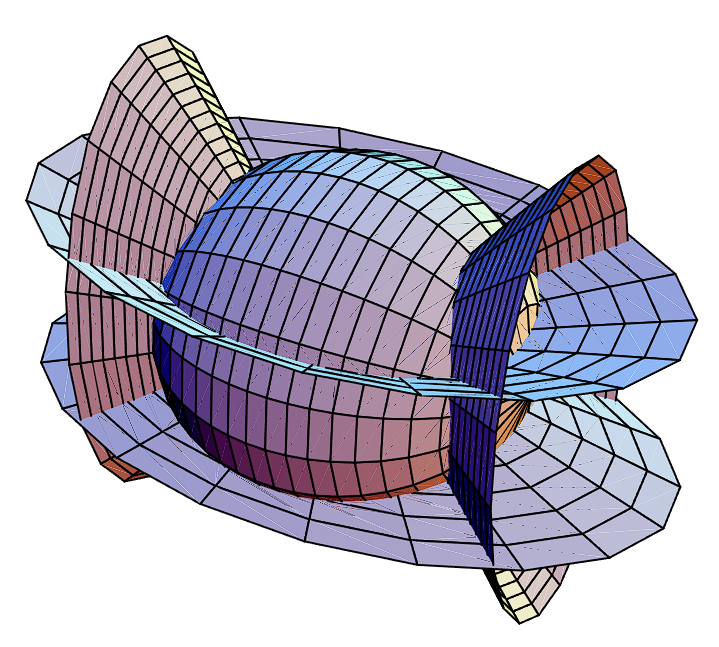
\includegraphics[width=\textwidth]{special_functions_fig/ellipsoidal_coordinates_schematic_diagram.png}
	\end{subfigure}
	\hfill
	\begin{subfigure}[b]{0.68\textwidth}
		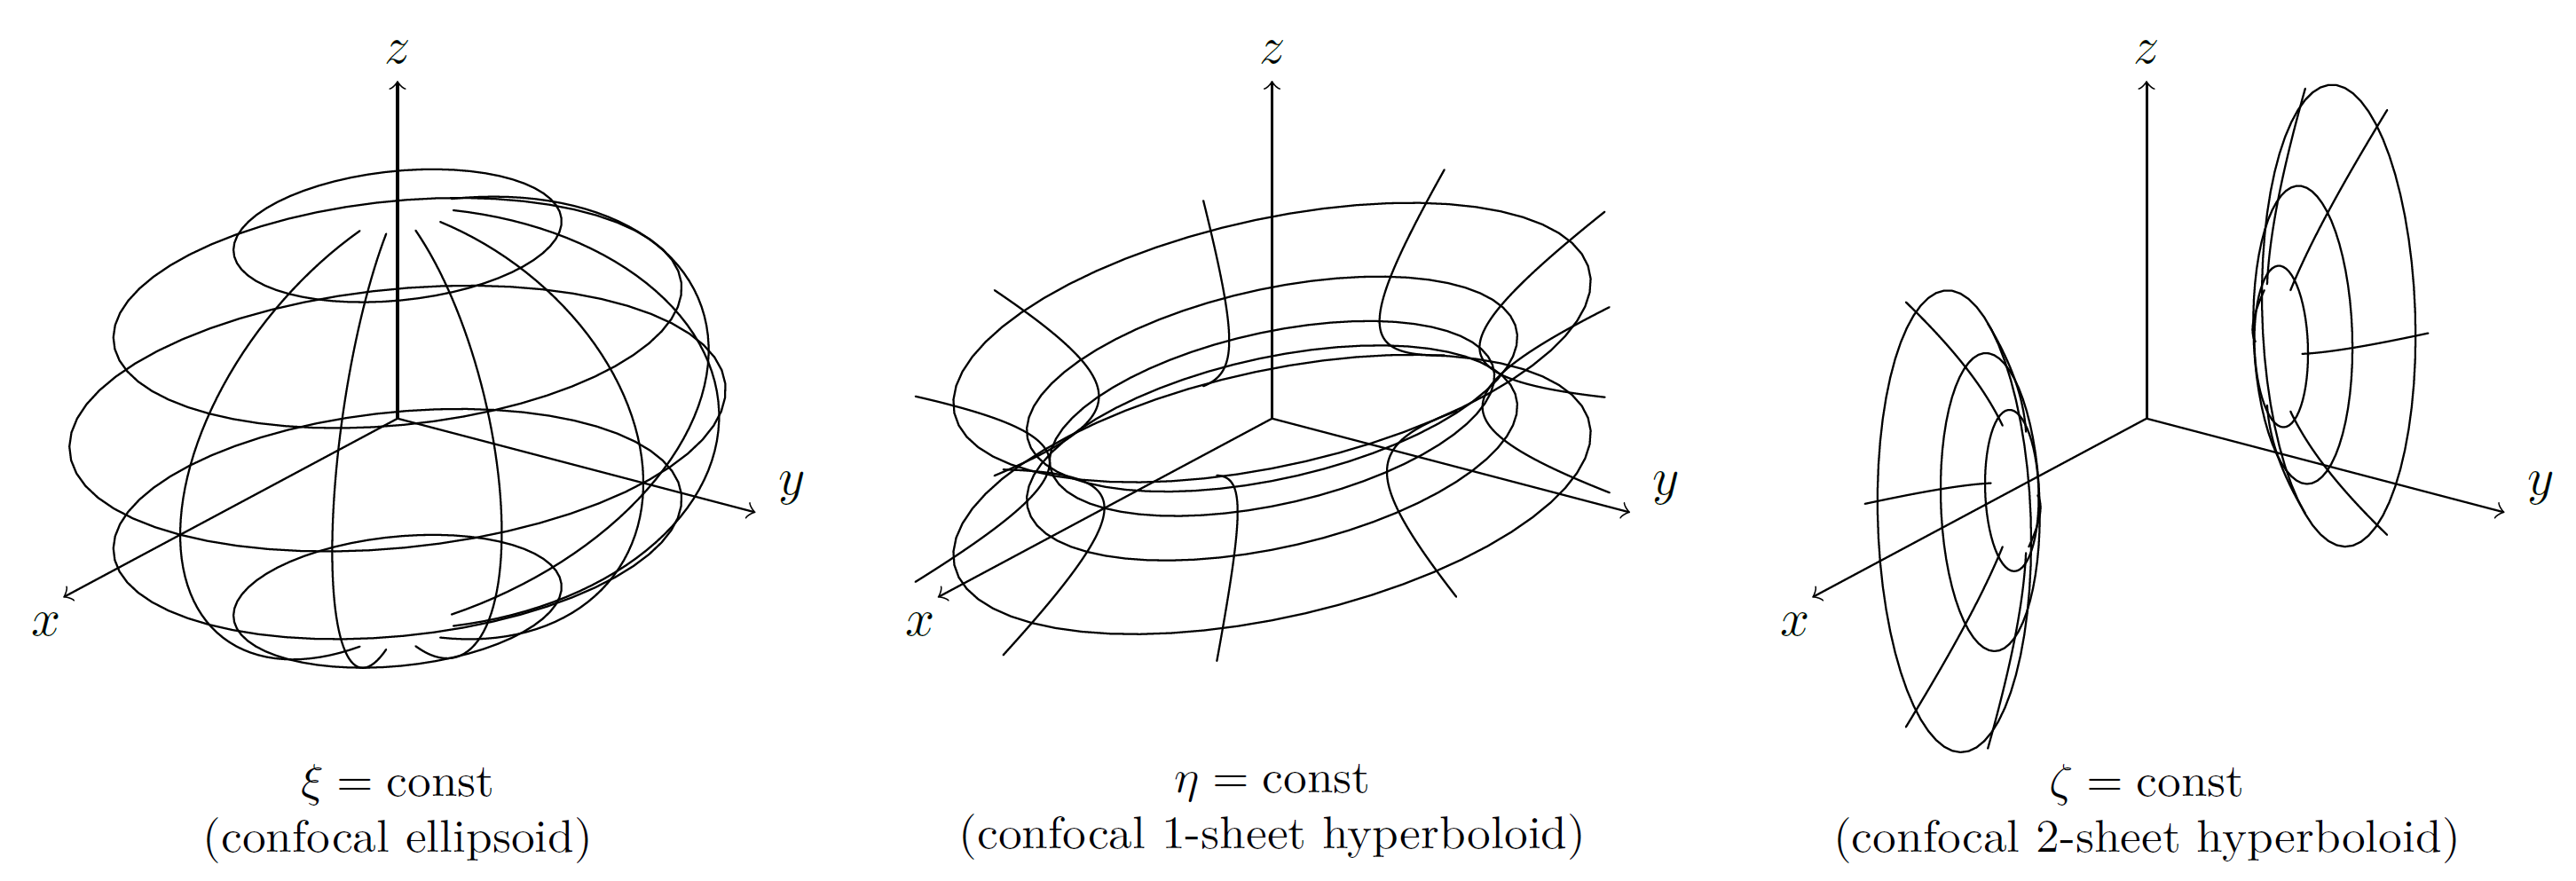
\includegraphics[width=\textwidth]{special_functions_fig/ellipsoidal_coordinates_schematic_diagram_2.png}
	\end{subfigure}
	\caption{椭球坐标示意图}
	\label{椭球坐标示意图}
\end{figure}

易知
\begin{align*}
	\frac{x^{2}}{a^{2}}+\frac{y^{2}}{b^{2}}+\frac{z^{2}}{c^{2}}
	 & =1+\frac{\xi\,\eta\,\zeta}{a^{2}b^{2}c^{2}},                                             \\
	\xi\,\eta+\eta\,\zeta+\zeta\,\xi
	 & =a^{2}b^{2}c^{2}\Bigl(\frac{x^{2}}{a^{4}}+\frac{y^{2}}{b^{4}}+\frac{z^{2}}{c^{4}}\Bigr),
\end{align*}
\(-c^{2}\le\xi<0\) 对应椭球\((a,b,c)\)的内部；\(\xi>0\) 对应椭球外部；\(\xi=0\) 对应椭球表面.

易证，椭球坐标系是正交系，其距离元为
\begin{equation*}
	\d s^{2}=\d x^{2}+\d y^{2}+\d z^{2}
	=h_{\xi}^{2}\,\d \xi^{2}+h_{\eta}^{2}\,\d \eta^{2}+h_{\zeta}^{2}\,\d \zeta^{2},
\end{equation*}
其中
\begin{align*}
	 & h_{\xi}=\frac12\sqrt{\frac{(\xi-\eta)(\xi-\zeta)}{\varphi(\xi)}},\quad
	h_{\eta}=\frac12\sqrt{\frac{(\eta-\xi)(\eta-\zeta)}{\varphi(\eta)}},\quad
	h_{\zeta}=\frac12\sqrt{\frac{(\zeta-\xi)(\zeta-\eta)}{\varphi(\zeta)}}    \\
	 & \varphi(\Theta)=(a^{2}+\Theta)(b^{2}+\Theta)(c^{2}+\Theta).
\end{align*}

进而体积元为
\begin{equation*}
	\d V
	=h_{\xi}\,h_{\eta}\,h_{\zeta}\,\d \xi\, \d \eta\, \d \zeta=-\frac{(\xi-\eta)(\eta-\zeta)(\zeta-\xi)}
	{8\sqrt{-\varphi(\xi)\,\varphi(\eta)\,\varphi(\zeta)}}\,
	\d \xi\,\d \eta\,\d \zeta.
\end{equation*}

拉普拉斯算子为
\begin{equation*}
	\nabla^{2}
	=\frac{4\sqrt{\varphi(\xi)}}{(\xi-\eta)(\xi-\zeta)}
	\frac{\partial}{\partial\xi}\Bigl(\sqrt{\varphi(\xi)}\,
	\frac{\partial}{\partial\xi}\Bigr)\nonumber
	-\frac{4\sqrt{-\varphi(\eta)}}{(\eta-\xi)(\eta-\zeta)}
	\frac{\partial}{\partial\eta}\Bigl(\sqrt{-\varphi(\eta)}\,
	\frac{\partial}{\partial\eta}\Bigr)\nonumber
	+\frac{4\sqrt{\varphi(\zeta)}}{(\zeta-\xi)(\zeta-\eta)}
	\frac{\partial}{\partial\zeta}\Bigl(\sqrt{\varphi(\zeta)}\,
	\frac{\partial}{\partial\zeta}\Bigr).
\end{equation*}

基矢为
\begin{align*}
	\uv{e}_{\xi}
	 & =\frac{1}{h_{\xi}}\frac{\partial\vb{r}}{\partial\xi}
	=\frac{1}{2h_{\xi}}\Bigl(\frac{x}{a^{2}+\xi}\uv{e}_{x}
	+\frac{y}{b^{2}+\xi}\uv{e}_{y}
	+\frac{z}{c^{2}+\xi}\uv{e}_{z}\Bigr),\notag                 \\
	\uv{e}_{\eta}
	 & =\frac{1}{h_{\eta}}\frac{\partial\vb{r}}{\partial\eta}
	=\frac{1}{2h_{\eta}}\Bigl(\frac{x}{a^{2}+\eta}\uv{e}_{x}
	+\frac{y}{b^{2}+\eta}\uv{e}_{y}
	+\frac{z}{c^{2}+\eta}\uv{e}_{z}\Bigr),\notag                \\
	\uv{e}_{\zeta}
	 & =\frac{1}{h_{\zeta}}\frac{\partial\vb{r}}{\partial\zeta}
	=\frac{1}{2h_{\zeta}}\Bigl(\frac{x}{a^{2}+\zeta}\uv{e}_{x}
	+\frac{y}{b^{2}+\zeta}\uv{e}_{y}
	+\frac{z}{c^{2}+\zeta}\uv{e}_{z}\Bigr).
\end{align*}

易知，\(\uv{e}_{\Theta}\;(\Theta=\xi/\,\eta/\,\zeta)\) 恰为等 \(\Theta\) 面
\begin{equation*}
	\frac{x^{2}}{a^{2}+\Theta}+\frac{y^{2}}{b^{2}+\Theta}+\frac{z^{2}}{c^{2}+\Theta}=1
\end{equation*}
的单位法向量，\(\uv{e}_{\xi}|_{\xi=0}\)恰为原椭球表面的外法向量.

若某函数恰可分离变量为形式
\(\Psi(\xi,\eta,\zeta)=f(\xi,\eta,\zeta)\,g(\xi)\)，则
\begin{equation*}
	\nabla^{2}\Psi
	=g\,\nabla^{2}f
	+\frac{4\,f\,\sqrt{\varphi(\xi)}}{(\xi-\eta)(\xi-\zeta)}
	\Bigl[
		2\frac{\partial f}{\partial\xi}\frac{1}{f}\,
		\sqrt{\varphi(\xi)}\,\frac{\d g}{\d \xi}
		+\frac{\d}{\d \xi}\Bigl(\sqrt{\varphi(\xi)}\,\frac{\d g}{\d \xi}\Bigr)
		\Bigr].
\end{equation*}

\newpage
\section{Mathieu函数}
\subsection{一般形式}
Mathieu方程形如
\begin{equation*}
	\frac{\d^2 y}{\d z^2} + (\lambda - 2q \cos(2z)) y = 0.
\end{equation*}
展开为Floquent解
\begin{equation*}
	y(z) = \sum_{k=-\infty}^{\infty} c_k e^{i(\nu + 2k)z}
\end{equation*}

代入得临项系数递推关系
\begin{equation*}
	c_{k+1} - \frac{D_k}{q} c_k + c_{k-1} = 0, \quad D_k = \lambda - (\nu + 2k)^2.
\end{equation*}

写成无穷连分式，即
\begin{equation*}
	\frac{c_k}{c_{k-1}} = \frac{q}{D_k - \dfrac{q^2}{D_{k+1} - \dfrac{q^2}{D_{k+2} - \dots}}}, \quad \frac{c_{k-1}}{c_k} = \frac{q}{D_{k-1} - \dfrac{q^2}{D_{k-2} - \dfrac{q^2}{D_{k-3} - \dots}}}.
\end{equation*}
\begin{equation*}
	D_k - \frac{q^2}{D_{k+1} - \dfrac{q^2}{D_{k+2} - \dots}} = \frac{q^2}{D_{k-1} - \dfrac{q^2}{D_{k-2} - \dfrac{q^2}{D_{k-3} - \dots}}}.
\end{equation*}
\begin{equation*}
	\lambda - (\nu + 2k)^2 - \frac{q^2}{\lambda - (\nu + 2k + 2)^2 - \dfrac{q^2}{\lambda - (\nu + 2k + 4)^2 - \dots}} = \frac{q^2}{\lambda - (\nu + 2k - 2)^2 - \dfrac{q^2}{\lambda - (\nu + 2k - 4)^2 - \dots}}.
\end{equation*}

对 \(\nu = 2n\)（\(n \in \mathbb{N}\)）的全周期解：

若 \(c_{-n}\) 有限，由 \(\left( \dfrac{c_{-n}}{c_{-n-1}} \right) \left( \dfrac{c_{-n-1}}{c_{-n}} \right) = 1\) 得
\begin{align*}
	 & \lambda - 4 - \frac{2q^2}{\lambda} = \frac{q^2}{\lambda - 16 - \dfrac{q^2}{\lambda - 36 - \dots}}                                                                                                       \\
	 & \implies \lambda - (2n)^2 - \frac{q^2}{\lambda - (2n - 2)^2 - \dots - \dfrac{q^2}{\lambda - 4 - \dfrac{2q^2}{\lambda}}} = \frac{q^2}{\lambda - (2n + 2)^2 - \dfrac{q^2}{\lambda - (2n + 4)^2 - \dots}}.
\end{align*}
该式解记为 \(\lambda = a_{2n}(q)\)，对应系数满足 \(c_{-n-l} = c_{-n+l}\)（\(l \in \mathbb{N}\)），进而
\begin{equation*}
	y = \mathrm{ce}_{2n}(z) = \sum_{s=-\infty}^{\infty} c_{s-n} e^{2isz} = c_{-n} + 2 \sum_{s=1}^{\infty} c_{s-n} \cos(2sz)
\end{equation*}

若 \(c_{-n} = 0\)，由临项递推式得
\begin{align*}
	 & \lambda - 4 = \frac{q^2}{\lambda - 16 - \dfrac{q^2}{\lambda - 36 - \dots}}                                                                                                      \\
	 & \implies \lambda - (2n + 2)^2 - \frac{q^2}{\lambda - (2n)^2 - \dots - \dfrac{q^2}{\lambda - 4}} = \frac{q^2}{\lambda - (2n + 4)^2 - \dfrac{q^2}{\lambda - (2n + 6)^2 - \dots}}.
\end{align*}
该式解记为 \(\lambda = b_{2n+2}(q)\)，对应系数满足 \(c_{-n-l} = -c_{-n+l}\)（\(l \in \mathbb{N}\)），进而
\begin{equation*}
	y = \mathrm{se}_{2n+2}(z) = \sum_{s=-\infty}^{\infty} c_{s-n} e^{2isz} = -2i \sum_{s=0}^{\infty} c_{s-n-1} \sin((2s + 2)z)
\end{equation*}

对 \(\nu = 2n + 1\)（\(n \in \mathbb{N}\)）的半周期解：
由 \(\left( \dfrac{c_{-n}}{c_{-n-1}} \right) \left( \dfrac{c_{-n-1}}{c_{-n}} \right) = 1\) 得
\begin{equation*}
	\lambda - 1 - \frac{q^2}{\lambda - 9 - \dfrac{q^2}{\lambda - 25 - \dots}} = \frac{q^2}{\lambda - 1 - \dfrac{q^2}{\lambda - 9 - \dots}} = \pm q.
\end{equation*}
两支分别对应（\(l \in \mathbb{N}\)）
\begin{align*}
	 & \lambda = a_{2n+1}(q) = 1 + q + \frac{q^2}{\lambda - 9 - \dfrac{q^2}{\lambda - 25 - \dots}}, \quad c_{l-n} = c_{-l-n-1},      \\
	 & y = \mathrm{ce}_{2n+1}(z) = \sum_{s=-\infty}^{\infty} c_{s-n} e^{i(2s + 1)z} = 2 \sum_{s=0}^{\infty} c_{s-n} \cos((2s + 1)z).
\end{align*}
以及
\begin{align*}
	 & \lambda = b_{2n+1}(q) = 1 - q + \frac{q^2}{\lambda - 9 - \dfrac{q^2}{\lambda - 25 - \dots}}, \quad c_{l-n} = -c_{-l-n-1},      \\
	 & y = \mathrm{se}_{2n+1}(z) = \sum_{s=-\infty}^{\infty} c_{s-n} e^{i(2s + 1)z} = 2i \sum_{s=0}^{\infty} c_{s-n} \sin((2s + 1)z).
\end{align*}

Mathieu方程的解也可统一写作
\begin{align*}
	 & \mathrm{ce}_{2n}(z, q) = \sum_{r=0}^{\infty} A_{2r}^{2n} \cos(2rz), \quad
	\mathrm{se}_{2n}(z, q) = \sum_{r=0}^{\infty} B_{2r+2}^{2n} \sin((2r + 2)z).              \\
	 & \mathrm{ce}_{2n+1}(z, q) = \sum_{r=0}^{\infty} A_{2r+1}^{2n+1} \cos((2r + 1)z), \quad
	\mathrm{se}_{2n+1}(z, q) = \sum_{r=0}^{\infty} B_{2r+1}^{2n+1} \sin((2r + 1)z).
\end{align*}

易见，有正交关系
\begin{equation*}
	\int_{0}^{2\pi} \mathrm{ce}_m(z, q) \mathrm{ce}_n(z, q) \,\d z = \int_{0}^{2\pi} \mathrm{se}_m(z, q) \mathrm{se}_n(z, q) \,\d z = 0, \quad m \neq n.
\end{equation*}
\begin{equation*}
	\int_{0}^{2\pi} \mathrm{ce}_m(z, q) \mathrm{se}_n(z, q) \,\d z = 0.
\end{equation*}

另外，规定各系数的归一化关系为
\begin{equation*}
	\frac{1}{\pi} \int_{0}^{2\pi} \mathrm{ce}_m^2(z, q) \,\d z = \frac{1}{\pi} \int_{0}^{2\pi} \mathrm{se}_m^2(z, q) \,\d z = 1.
\end{equation*}
也即（适用于任何上标）
\begin{equation*}
	2|A_0|^2 + \sum_{r=1}^{\infty} |A_{2r}|^2 = \sum_{r=0}^{\infty} |A_{2r+1}|^2 = \sum_{r=0}^{\infty} |B_{2r+2}|^2 = \sum_{r=0}^{\infty} |B_{2r+1}|^2 = 1.
\end{equation*}

\subsection{特殊形式的函数展开}
显然，\(\lambda\)可以展开成\(q\)的幂级数，通常而言，只考虑\(q\)较小的情形。

易见
\begin{equation*}
	a_{2n}(0) = (2n)^2, \quad b_{2n}(0) = (2n + 2)^2, \quad a_{2n+1}(0) = b_{2n}(0) = (2n)^2.
\end{equation*}
\begin{align*}
	a_{2n}(q) - b_{2n}(q)     & = \frac{2q^{2n}}{((4n - 2)!!)^2} + \mathcal{O}(q^{2n+2}), \\
	a_{2n+1}(q) - b_{2n+1}(q) & = \frac{2q^{2n+1}}{((4n)!!)^2} + \mathcal{O}(q^{2n+2}).
\end{align*}
也可以写成 (\(m \in \mathbb{Z}^+\))
\begin{equation*}
	a_m(q) - b_m(q) = \frac{q^m}{2^{2m-3}((m - 1)!)^2} + \mathcal{O}(q^{m+1}).
\end{equation*}

具体精确到\(q^4\) 项，根据前决定\(\lambda(q)\) 的方程，展开得
\begin{align*}
	a_0 & = -\frac{1}{2}q^2 + \frac{7}{128}q^4 + \mathcal{O}(q^6).                                                                      \\
	b_1 & = 1 - q - \frac{1}{8}q^2 + \frac{1}{64}q^3 - \frac{1}{1536}q^4 + \mathcal{O}(q^5),                                            \\
	a_1 & = 1 + q - \frac{1}{8}q^2 - \frac{1}{64}q^3 - \frac{1}{1536}q^4 + \mathcal{O}(q^5).                                            \\
	b_2 & = 4 - \frac{1}{12}q^2 + \frac{5}{13824}q^4 + \mathcal{O}(q^6),                                                                \\
	a_2 & = 4 + \frac{5}{12}q^2 - \frac{763}{13824}q^4 + \mathcal{O}(q^6).                                                              \\
	b_3 & = 9 + \frac{1}{16}q^2 - \frac{1}{64}q^3 + \frac{13}{20480}q^4 + \mathcal{O}(q^5),                                             \\
	a_3 & = 9 + \frac{1}{16}q^2 + \frac{1}{64}q^3 + \frac{13}{20480}q^4 + \mathcal{O}(q^5).                                             \\
	b_4 & = 16 + \frac{1}{30}q^2 - \frac{317}{86400}q^4 + \mathcal{O}(q^6),                                                             \\
	a_2 & = 16 + \frac{1}{30}q^2 + \frac{433}{86400}q^4 + \mathcal{O}(q^6).                                                             \\
	b_m & \approx a_m = m^2 + \frac{q^2}{2(m^2 - 1)} + \frac{(5m^2 + 7)q^4}{32(m^2 - 1)^3(m^2 - 4)} + \mathcal{O}(q^5), \quad m \geq 5.
\end{align*}

类似地，对 \(\mathrm{ce}\), \(\mathrm{se}\) 函数展开至\(q^2\) 项。

对 \(m\geq4\) (\(m = 0, 1, 2, 3\)需要单独讨论), 根据递推式 (\(s \in \mathbb{Z}\))
\begin{equation*}
	(a_m - (m - 2s)^2) A_{m-2s}^m - q A_{m-2s+2}^m - q A_{m-2s-2}^m = 0.
\end{equation*}
\begin{equation*}
	(b_m - (m - 2s)^2) B_{m-2s}^m - q B_{m-2s+2}^m - q B_{m-2s-2}^m = 0.
\end{equation*}
得（其他\(A,\,B\)项为 \(q^3\) 量级，可忽略）
\begin{align*}
	\frac{A_{m\pm2}^m}{A_m^m} = \frac{B_{m\pm2}^m}{B_m^m} & = \mp \frac{q}{4(m\pm1)} + \mathcal{O}(q^3),       \\
	\frac{A_{m\pm4}^m}{A_m^m} = \frac{B_{m\pm4}^m}{B_m^m} & = \frac{q^2}{32(m\pm1)(m\pm2)} + \mathcal{O}(q^4).
\end{align*}
代入归一化条件得（事实上对\(m\geq3\)都成立）
\begin{align*}
	\mathrm{ce}_m(z, q) & = \cos(mz) - \frac{q}{4} \left( \frac{1}{m+1}\cos((m+2)z) - \frac{1}{m-1}\cos((m-2)z) \right)                                                                      \\
	                    & \quad+ \frac{q^2}{16} \left( \frac{\cos((m+4)z)}{2(m+1)(m+2)} + \frac{\cos((m-4)z)}{2(m-1)(m-2)} - \frac{m^2 + 1}{(m^2 - 1)^2}\cos(mz) \right)                     \\[4pt]
	\mathrm{se}_m(z, q) & = \sin(mz) - \frac{q}{4} \left( \frac{1}{m+1}\sin((m+2)z) - \frac{1}{m-1}\sin((m-2)z) \right)                                                                      \\
	                    & \quad+ \frac{q^2}{16} \left( \frac{\sin((m+4)z)}{2(m+1)(m+2)} + \frac{\sin((m-4)z)}{2(m-1)(m-2)} - \frac{m^2 + 1}{(m^2 - 1)^2}\sin(mz) \right) + \mathcal{O}(q^3).
\end{align*}

\(m<3\)的项为
\begin{align*}
	\mathrm{ce}_0(z, q) & = \frac{1}{\sqrt{2}} \left( 1 - \frac12 q\cos(2z) + \frac{q^2}{16} \left( \frac12 \cos(4z) - 1 \right) + \mathcal{O}(q^3) \right)                \\
	\mathrm{ce}_1(z, q) & = \cos(z) - \frac{q}{8}\cos(3z) + \frac{q^2}{64} \left( \frac13 \cos(5z) - \cos(3z) - \frac12 \cos(z) \right) + \mathcal{O}(q^3)                 \\
	\mathrm{se}_1(z, q) & = \sin(z) - \frac{q}{8}\sin(3z) + \frac{q^2}{64} \left( \frac13 \sin(5z) + \sin(3z) - \frac12 \sin(z) \right) + \mathcal{O}(q^3)                 \\
	\mathrm{ce}_2(z, q) & = \cos(2z) - \frac{q}{12} \left( \cos(4z) - 3 \right) + \frac{q^2}{96} \left( \frac14 \cos(6z) - \frac{19}{3}\cos(2z) \right) + \mathcal{O}(q^3) \\
	\mathrm{se}_2(z, q) & = \sin(2z) - \frac{q}{12}\sin(4z) + \frac{q^2}{96} \left( \frac14 \sin(6z) - \frac13 \sin(2z) \right) + \mathcal{O}(q^3).
\end{align*}

\begin{figure}[htbp]
	\centering
	\begin{subfigure}[b]{0.45\textwidth}
		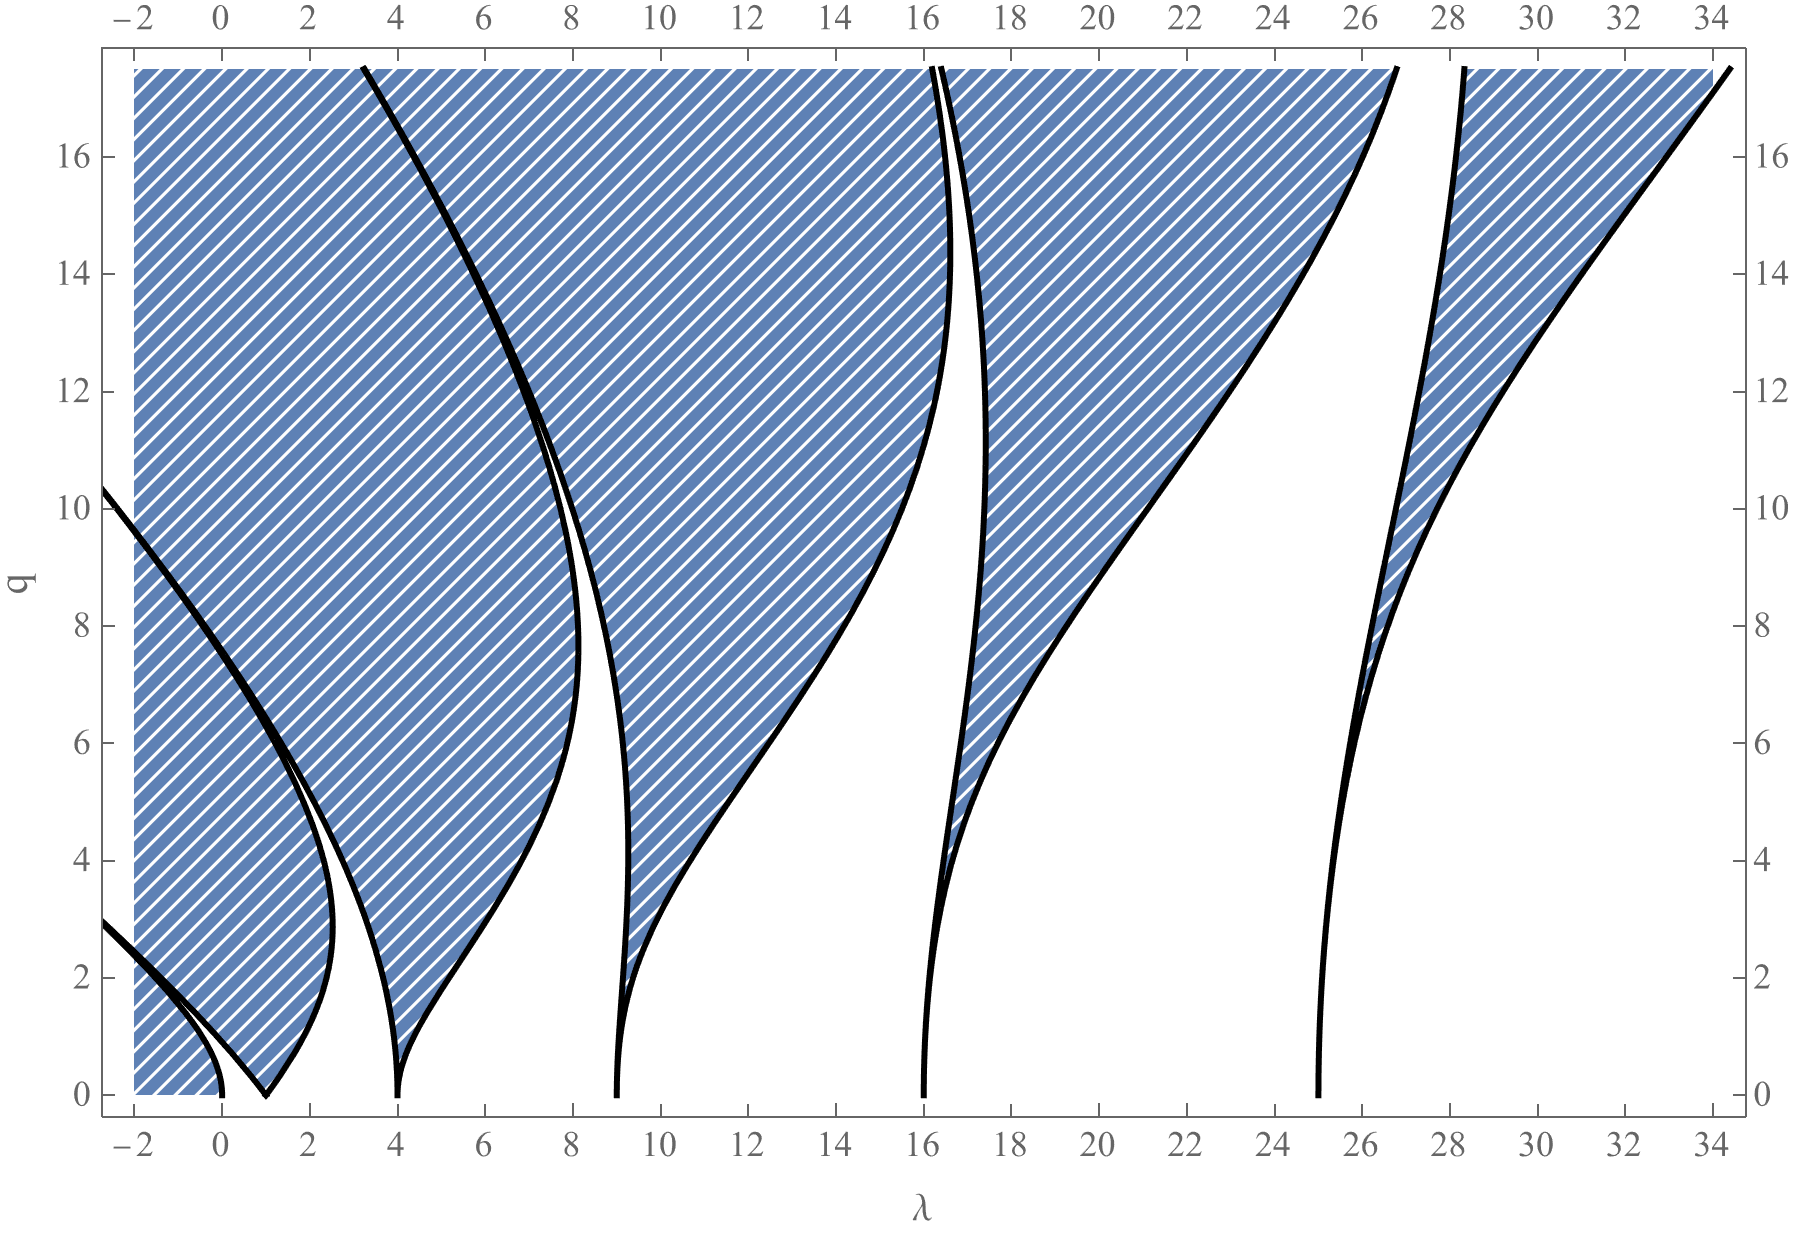
\includegraphics[width=\textwidth]{special_functions_fig/eigenvalue_curve_shaded_region_stable.png}
		\caption{本征值曲线（阴影区稳定）}
		\label{Mathieu方程解的示意图-本征值曲线(阴影区稳定)}
	\end{subfigure}
	\hfill
	\begin{subfigure}[b]{0.53\textwidth}
		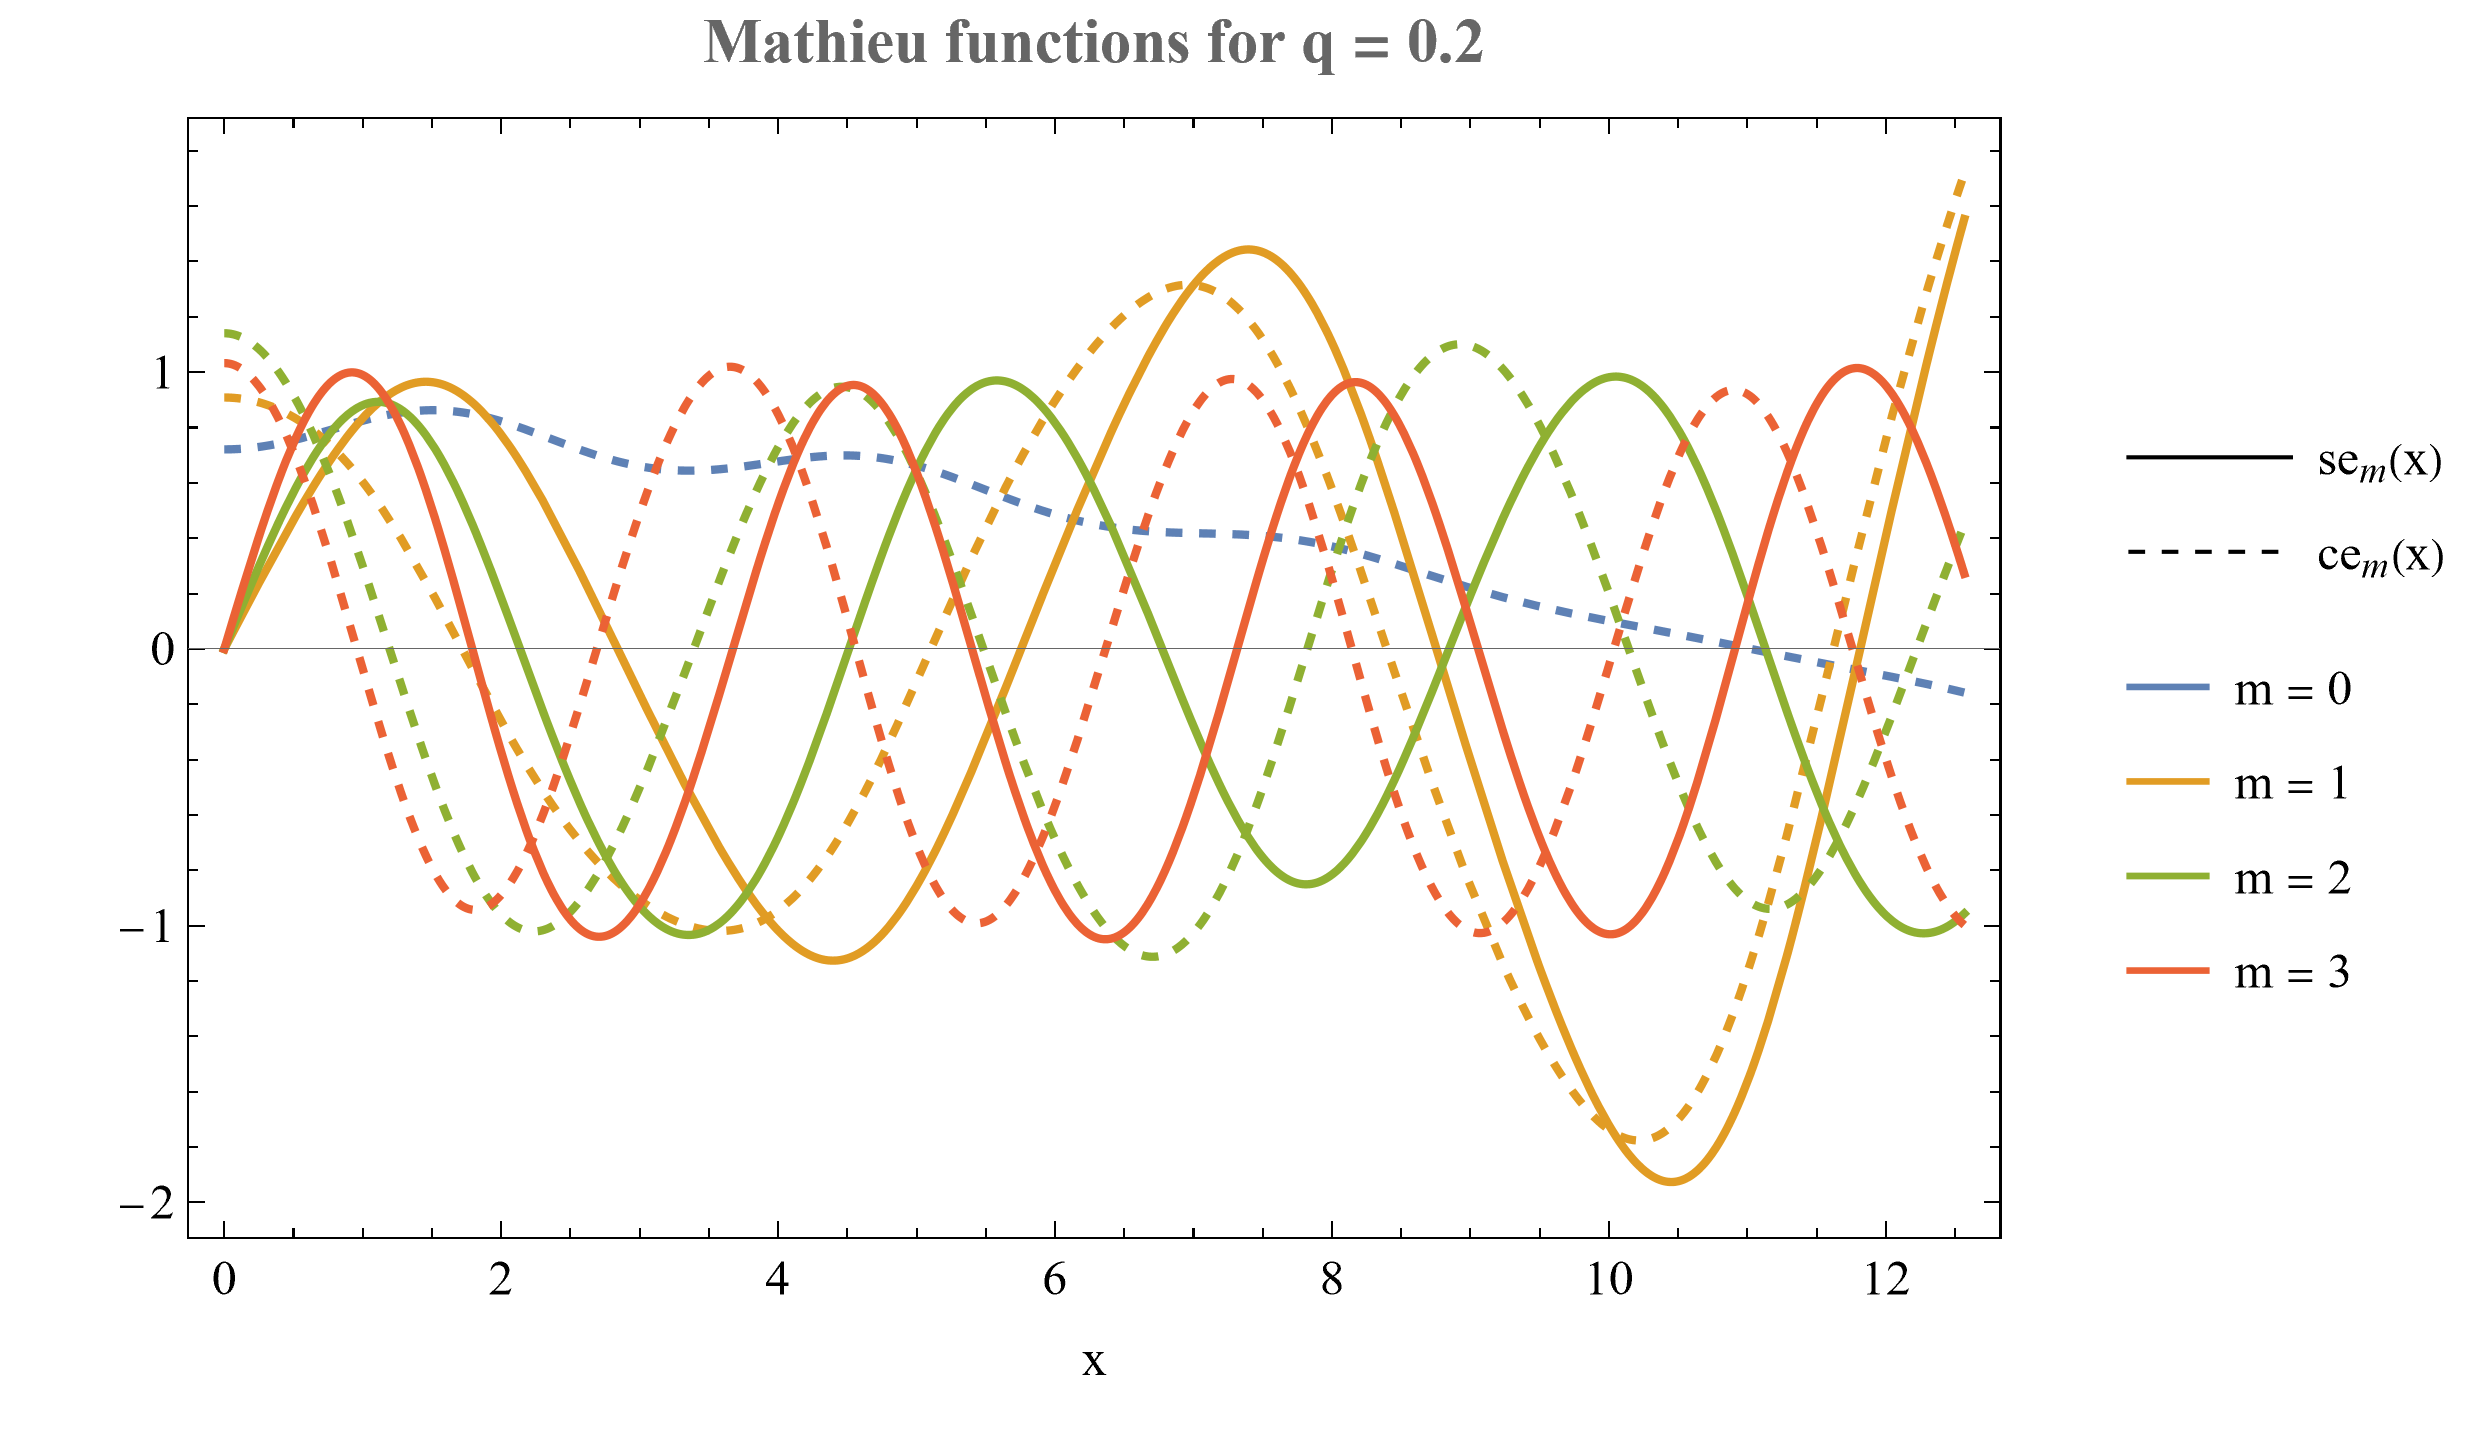
\includegraphics[width=\textwidth]{special_functions_fig/mathieu_function.png}
		\caption{Mathieu函数}
		\label{Mathieu方程解的示意图-Mathieu函数}
	\end{subfigure}
	\caption{Mathieu方程解的示意图}
	\label{Mathieu方程解的示意图}
\end{figure}

\newpage
\section{补充公式}
\subsection{傅里叶变换约定}
做傅里叶变换时，采用 \((2\pi)^{-1/2}\) 的对称因子，变换对 \(\vb{r} \leftrightarrow \vb{k}\), \(t \leftrightarrow \omega\) 约定为
\begin{equation*}
	F(\vb{r}, t) &= \frac{1}{(2\pi)^{2}} \int \d \vb{k} \int \d \omega \, F(\vb{k}, \omega) \, e^{i(\vb{k} \cdot \vb{r} - \omega t)}. \\
	F(\vb{k}, \omega) &= \frac{1}{(2\pi)^{2}} \int \d \vb{r} \int \d t \, F(\vb{r}, t) \, e^{-i(\vb{k} \cdot \vb{r} - \omega t)}. \\
\end{equation*}

下文考虑的 \(F(\vb{r}, t)\) 总是实的，\(\omega\) 的取值总是正的，因此
\begin{equation*}
	F(\vb{k}, -\omega) = F^{*}(\vb{k}, \omega), \quad
	\frac{1}{\sqrt{2\pi}} \int \d \omega \, e^{-i\omega t} = \frac{1}{\sqrt{2\pi}} \int_{0}^{\infty} \d \omega \, 2 \, \mathrm{Re} \, e^{-i\omega t}.
\end{equation*}

同时，与能量有关的积分，转换到频域取\(\omega > 0\) 部分，结果须乘2
\begin{equation*}
	\int F(\vb{r}, t) G(\vb{r}, t) \, \d t = 2 \int_{0}^{\infty} F(\vb{r}, \omega) G^{*}(\vb{r}, \omega) \, \d \omega.
\end{equation*}

在此列出文中常用的变换对
\begin{table}[htbp]
	\centering
	\begin{tabular}{|c|c|c|c|}
		\toprule
		\(f(\omega)\)                                    & \(f(\tau)\)                                             & \(f(\omega)\)                                  & \(f(\tau)\)                                                    \\
		\midrule
		\(\sqrt{2/\pi} \, K_{0}(a \omega)\)              & \(\dfrac{1}{\sqrt{\tau^{2} + a^{2}}}\)                  & \(\sqrt{\pi/2}H_{0}^{(1)}(a \omega)\)          & \(\dfrac{2 \Theta(\tau - a)}{\sqrt{\tau^{2} - a^{2}}}\)        \\[8pt]
		\(\sqrt{2/\pi} \, \omega K_{1}(a \omega)\)       & \(\dfrac{a}{(\tau^{2} + a^{2})^{3/2}}\)                 & \(\sqrt{\pi/2}\omega H_{0}^{(1)}(a \omega)\)   & \(-\dfrac{2 \tau \Theta(\tau - a)}{(\tau^{2} - a^{2})^{3/2}}\) \\[8pt]
		\(\sqrt{2/\pi} \, \omega^{2} K_{1}'(a \omega)\)  & \(\dfrac{\tau^{2} - 2a^{2}}{(\tau^{2} + a^{2})^{5/2}}\) & \(i \sqrt{\pi/2}\omega H_{1}^{(1)}(a \omega)\) & \(\dfrac{2 a \Theta(\tau - a)}{(\tau^{2} - a^{2})^{3/2}}\)     \\[8pt]
		\(i \sqrt{2/\pi} \, \omega^{2} K_{1}(a \omega)\) & \(\dfrac{3 a \tau}{(\tau^{2} + a^{2})^{5/2}}\)          &                                                &                                                                \\
		\bottomrule
	\end{tabular}
\end{table}

\subsection{多对数函数}

在玻色费米气体统计中，将玻色费米积分函数的定义为
\begin{equation*}
	g_{\nu}(z) &= \mathrm{Li}_{\nu}(z) = \dfrac{1}{\Gamma(\nu)} \int_{0}^{\infty} \dfrac{x^{\nu-1}}{z^{-1} e^{x} - 1} \, \d x = -\dfrac{1}{\Gamma(\nu)} \int_{0}^{\infty} x^{\nu-2} \ln(1 - z e^{-x}) \, \d x. \\
	f_{\nu}(z) &= -\mathrm{Li}_{\nu}(-z) = \dfrac{1}{\Gamma(\nu)} \int_{0}^{\infty} \dfrac{x^{\nu-1}}{z^{-1} e^{x} + 1} \, \d x = \dfrac{1}{\Gamma(\nu)} \int_{0}^{\infty} x^{\nu-2} \ln(1 + z e^{-x}) \, \d x. \\
\end{equation*}
其中\(\mathrm{Li}_{\nu}(z) \)是多对数函数，满足
\begin{equation*}
	\mathrm{Li}_{\nu}(z) = \sum_{k=1}^{\infty} \dfrac{z^{k}}{k^{\nu}},\quad \dfrac{\d  \mathrm{Li}_{\nu}(z)}{\d  z} = \dfrac{\mathrm{Li}_{\nu-1}(z)}{z}
\end{equation*}

根据多对数函数的性质，玻色/费米积分函数在特殊值下的展开为
\begin{equation*}
	&g_{\nu}(z) \big|_{z \to 1^{-}} =
	\begin{cases}
		\zeta(\nu) - \zeta(\nu-1) (1 - z) + \mathcal{O}((1-z)^{2}),              & \nu > 2.             \\[4pt]
		\zeta(2) + (1 - z) (\ln(1 - z) - 1) + \mathcal{O}((1-z)^{2} \ln(1 - z)), & \nu = 2.             \\[4pt]
		\zeta(\nu) + \Gamma(1-\nu) (1 - z)^{\nu-1} + \mathcal{O}(1 - z),         & \nu < 2, \nu \neq 1. \\[4pt]
		-\ln(1 - z),                                                             & \nu = 1.
	\end{cases}\\
	&f_{\nu}(z) \big|_{z \gg 1} = \dfrac{(\ln z)^{\nu}}{\Gamma(\nu+1)} + \dfrac{\pi^{2}}{6} \dfrac{(\ln z)^{\nu-2}}{\Gamma(\nu-1)} + \dfrac{7\pi^{4}}{360} \dfrac{(\ln z)^{\nu-4}}{\Gamma(\nu-3)} + \cdots.
\end{equation*}


\subsection{高维空间的球}

\(d\)维空间的立体角元为
\begin{equation*}
	\d \Omega_{d} = \prod_{i=1}^{d-1} (\sin\theta_{i})^{d-1-i} \, \d \theta_{i}, \quad 0 \le \theta_{j} \le \pi \ (j = 1, 2, \ldots, d-2), \quad 0 \le \theta_{d-1} \le 2\pi.
\end{equation*}
积分得总立体角以及沿某一方向的投影因子为
\begin{equation*}
	\Omega_{d} =\int\d\Omega_d \dfrac{2\pi^{d/2}}{\Gamma(d/2)},\quad \mathcal{P}_d=\frac{1}{\Omega_d}\int_{\theta_1\leq\pi/2}\cos\theta_1\d\Omega_d=\frac{\Omega_{d-1}}{(d-1)\Omega_d}.
\end{equation*}
式中用到
\begin{equation*}
	\int_{0}^{\pi} \sin^{n}\theta \, \d \theta = \sqrt{\pi} \dfrac{\Gamma\left( \dfrac{n+1}{2} \right)}{\Gamma\left( \dfrac{n+2}{2} \right)}
\end{equation*}
进而\(d\)维空间单位半径球的表面积为\(\Omega_d\)，体积为\(V_d=\Omega_d/d\)。

各向同性函数向波矢空间的傅里叶变换为
\begin{equation*}
	\int_{\mathbb{R}^{d}} f(r) e^{i \vb{k} \cdot \vb{r}} \, \d \vb{r} = (2\pi)^{d/2} k^{1-d/2} \int_{0}^{\infty} f(r) r^{d/2} J_{d/2-1}(kr) \, \d r.
\end{equation*}

运用该公式，得到\(d\)维自由空间的Helmholtz方程的格林函数解为
\begin{equation*}
	&(\nabla^{2} + k^{2}) G(\vb{R}) = \delta^{(d)}(\vb{R}), \quad \vb{R} = \vb{r} - \vb{r}'.\\
	&\implies\quad G(\vb{R}) = \int_{\mathbb{R}^{d}} \dfrac{\d \vb{q}}{(2\pi)^{d}} \dfrac{e^{i \vb{q} \cdot \vb{R}}}{q^{2} + k^{2}} = \dfrac{1}{2\pi} \left( \dfrac{k}{2\pi R} \right)^{d/2 - 1} K_{d/2 - 1}(kR).
\end{equation*}

根据第二类修正贝塞尔函数的展开式 (\(\mathcal{O}\) 指对应\(\nu\)范围下，下一个展开项的最大可能阶数)
\begin{equation*}
	K_{\nu}(x) \big|_{x \gg 1} = \sqrt{\dfrac{\pi}{2x}} e^{-x} \left( 1 + \dfrac{4\nu^{2} - 1}{8x} + \mathcal{O}(x^{-2}) \right), \quad K_{\nu}(x) \big|_{x \ll 1} =
	\begin{cases}
		\dfrac{1}{2} \Gamma(|\nu|) \left( \dfrac{x}{2} \right)^{-|\nu|} + \mathcal{O}(x^{2-|\nu|} \ln x), & \nu \neq 0. \\[6pt]
		-\ln \dfrac{x}{2} - \gamma_{E} + \mathcal{O}(x^{2}),                                              & \nu = 0.
	\end{cases}
\end{equation*}

得到
\begin{equation*}
	&G(\vb{R}) \big|_{kR \gg 1} = \dfrac{1}{\sqrt{8\pi k R}} \left( \dfrac{k}{2\pi R} \right)^{d/2 - 1} e^{-kR} \left( 1 + \dfrac{4\nu^{2} - 1}{8 k R} + \mathcal{O}((kR)^{-2}) \right).\\[6pt]
	&G(\vb{R}) \big|_{kR \ll 1} =
	\begin{cases}
		\displaystyle \dfrac{\Gamma\left(d/2 - 1 \right)}{4\pi^{d/2} R^{d-2}} + \mathcal{O}\left( (kR)^{4-d} \ln(kR) \right),     & d > 2. \\[10pt]
		\displaystyle \dfrac{1}{2\pi} \left( -\ln \dfrac{kR}{2} - \gamma_{E} \right) + \mathcal{O}\left( (kR)^{2} \right),        & d = 2. \\[10pt]
		\displaystyle \dfrac{\Gamma\left( 1 - d/2 \right)}{2^{d} \pi^{d/2}} k^{d-2} + \mathcal{O}\left( (kR)^{2} \ln(kR) \right), & d < 2.
	\end{cases}
\end{equation*}

\begin{figure}[htbp]
	\centering
	\begin{minipage}[b]{0.49\textwidth}
		\centering
		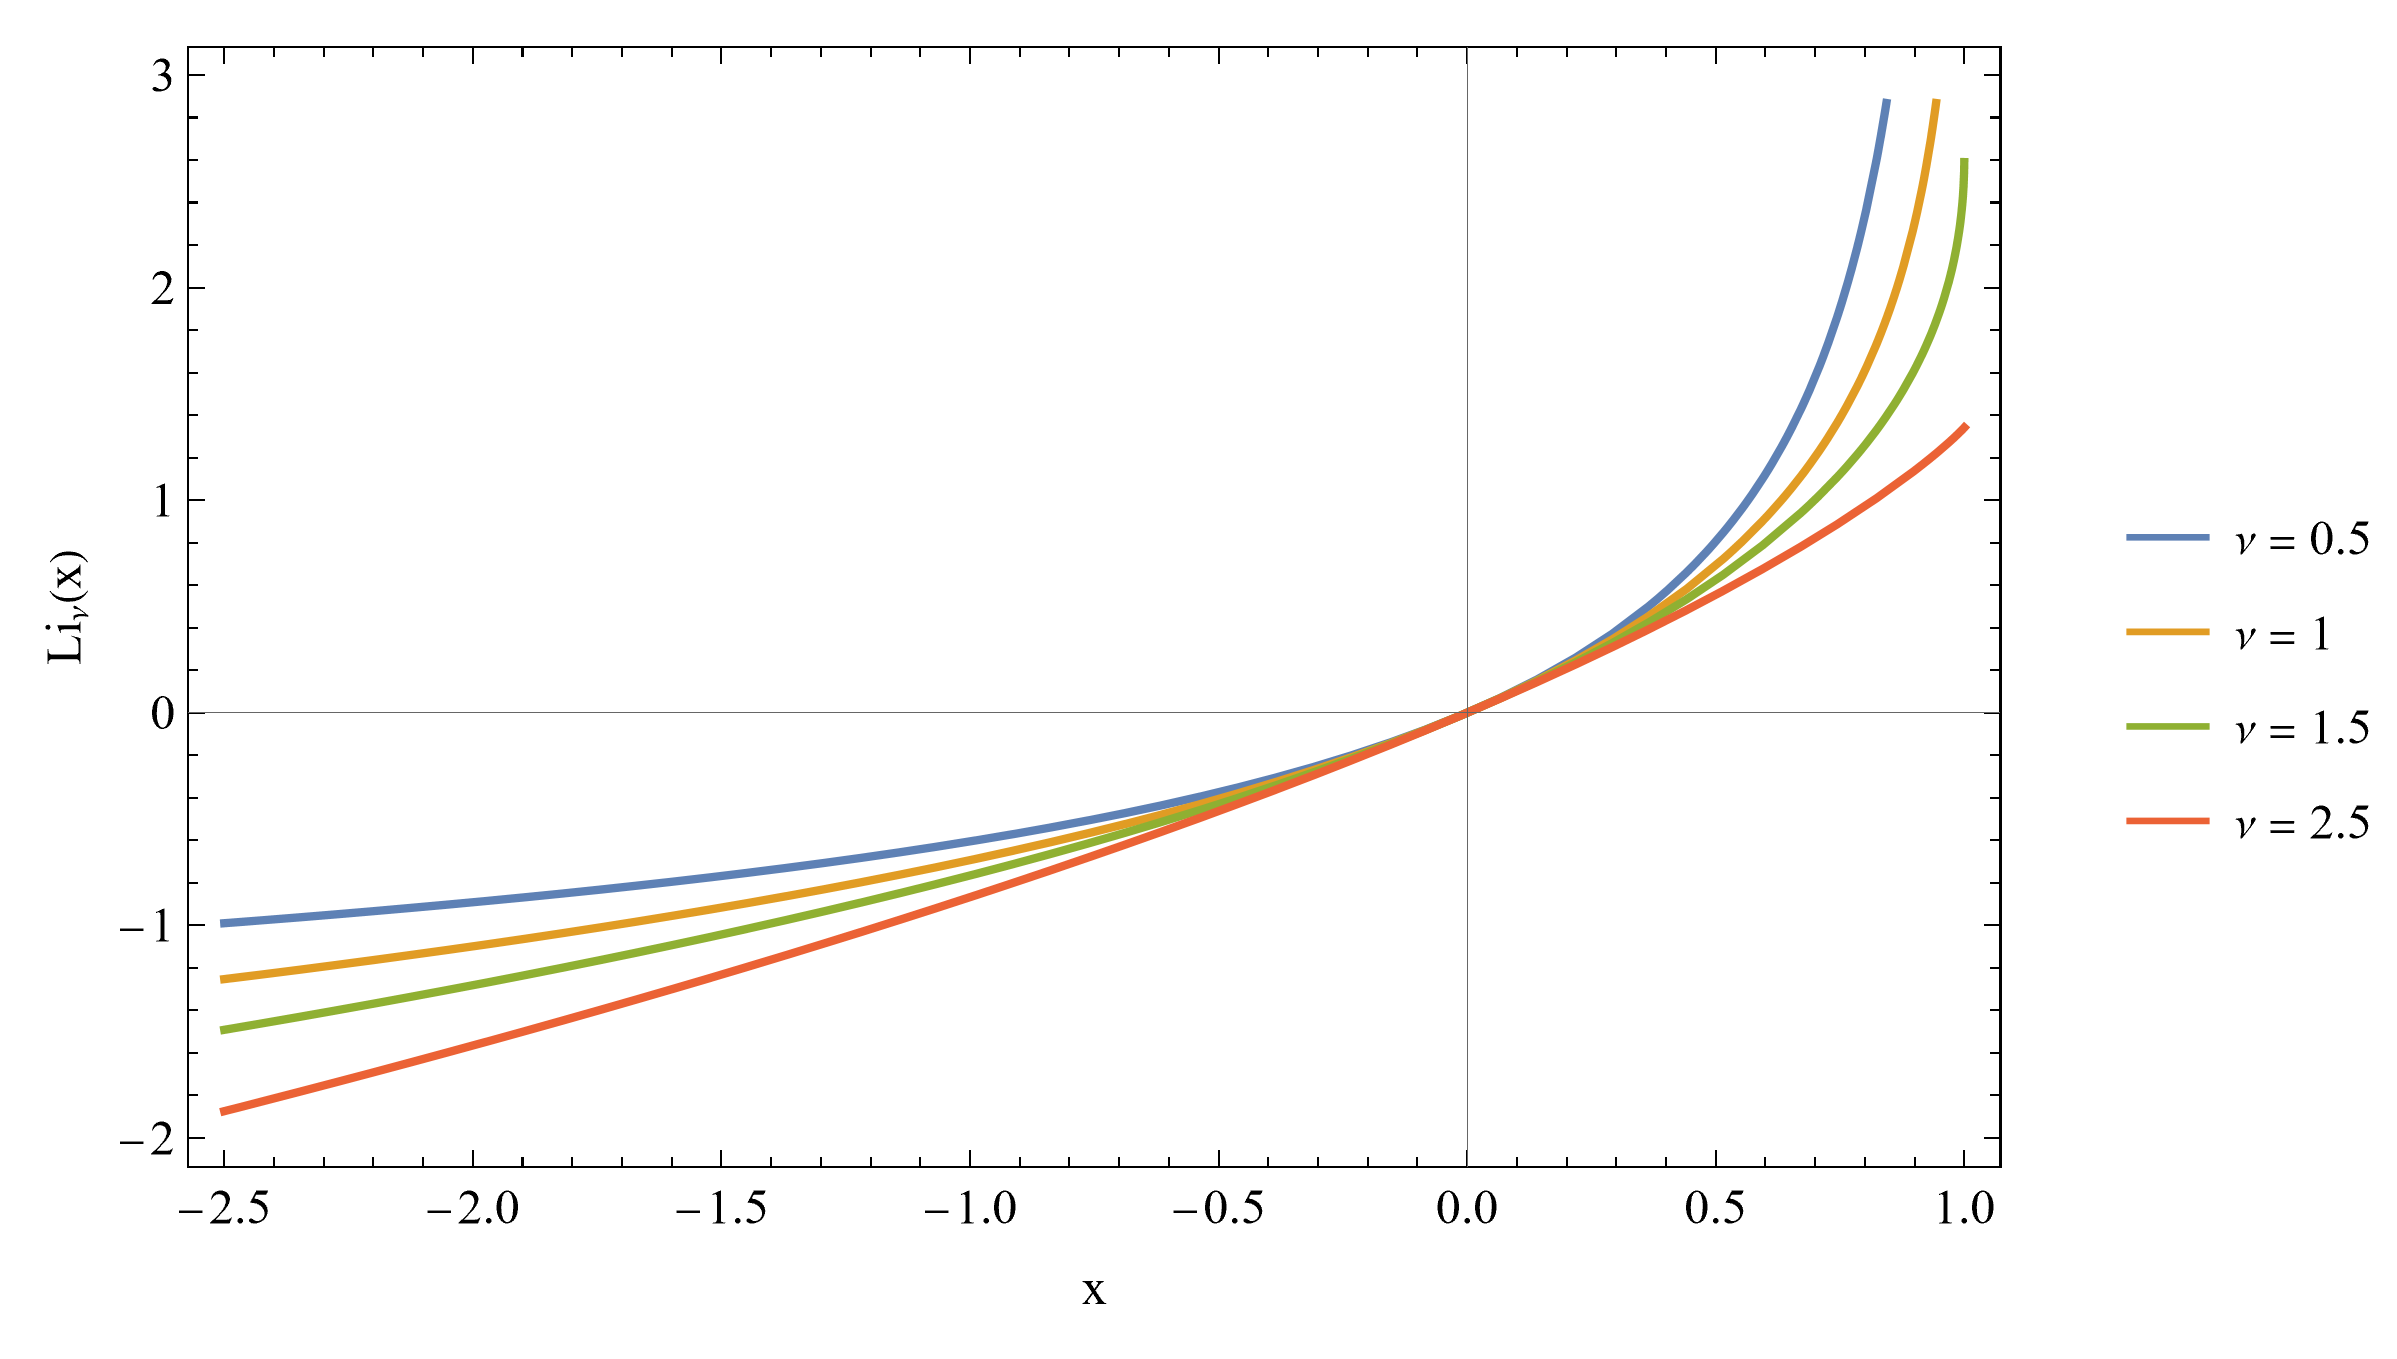
\includegraphics[width=\textwidth]{special_functions_fig/polylogarithm_function.png}
		\caption{多对数函数}
		\label{多对数函数}
	\end{minipage}
	\hfill
	\begin{minipage}[b]{0.49\textwidth}
		\centering
		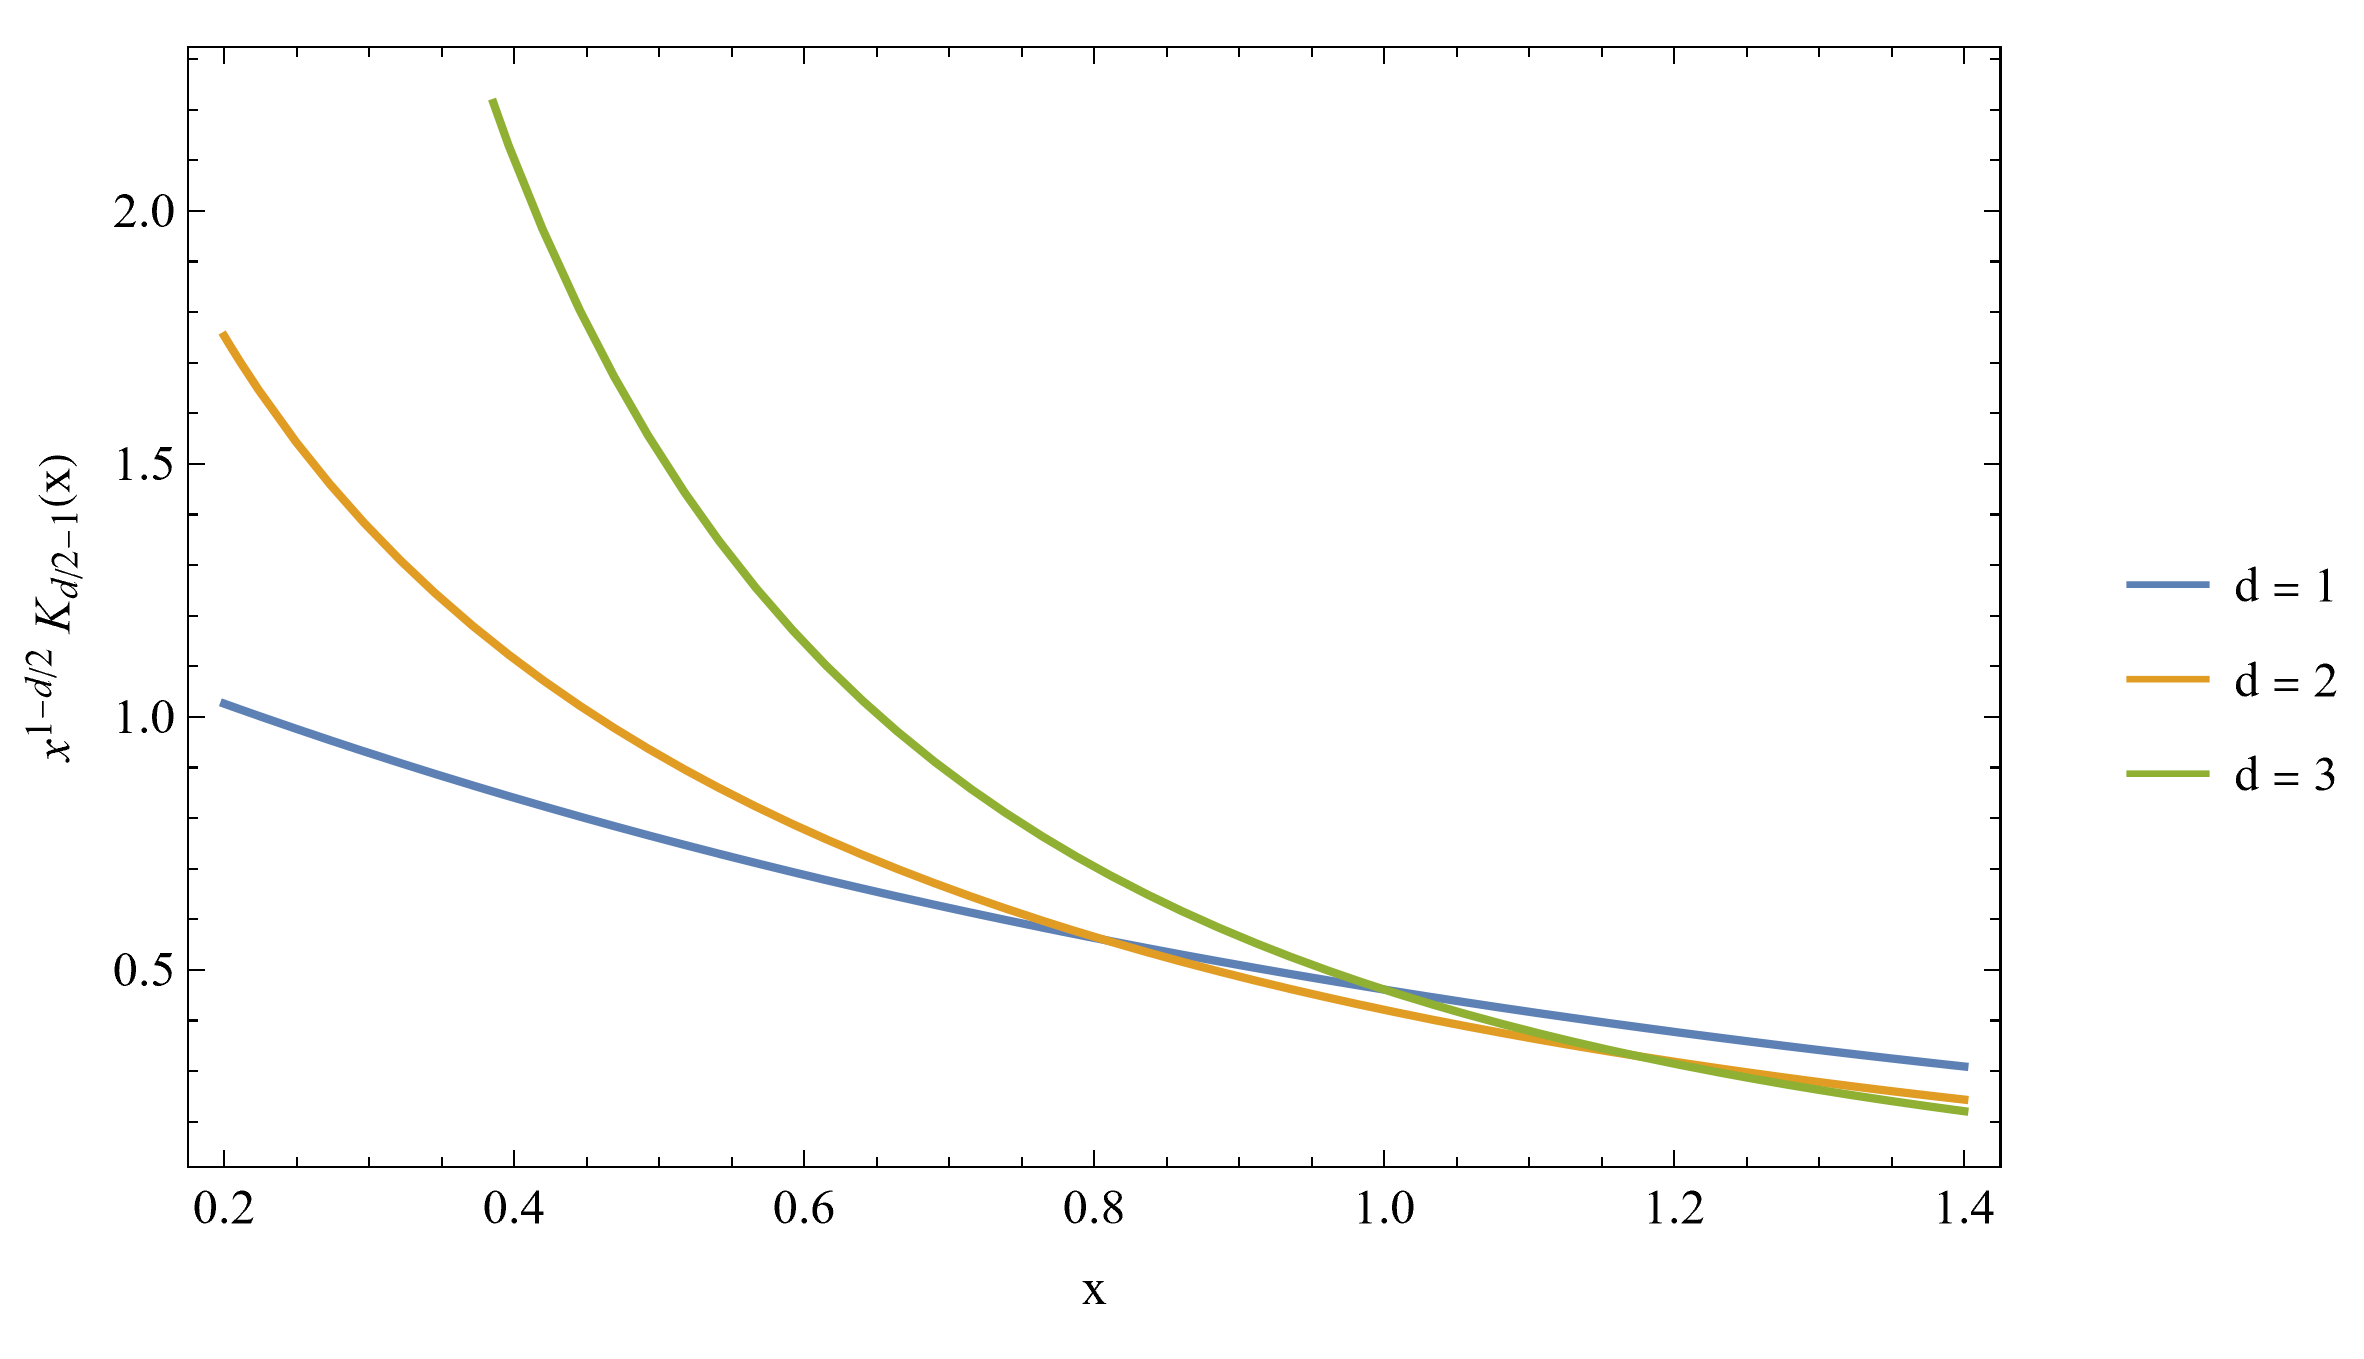
\includegraphics[width=\textwidth]{special_functions_fig/high_dimensional_helmholtz_equation_green_function.png}
		\caption{高维空间Helmholtz方程的格林函数}
		\label{高维空间Helmholtz方程的格林函数}
	\end{minipage}
\end{figure}

\subsection{数学公式}
与修正Hankel变换有关的积分恒等式
\begin{equation*}
	&\int_{0}^{\infty} \rho J_{0}(a\rho) K_{0}(\lambda\rho) \, \d \rho = \frac{1}{a^{2} + \lambda^{2}}, \quad
	\int_{0}^{\infty} \rho J_{1}(a\rho) K_{1}(\lambda\rho) \, \d \rho = \frac{a}{\lambda (a^{2} + \lambda^{2})}, \\
	&\int_{0}^{\infty} \left[ \frac{K_{1}(\lambda\rho)}{\lambda\rho} \left( J_{0}(a\rho) + J_{2}(a\rho) \right) + K_{1}'(\lambda\rho) \left( J_{0}(a\rho) - J_{2}(a\rho) \right) \right] \rho \, \d \rho = \frac{a^{2} - \lambda^{2}}{\lambda^{2} (a^{2} + \lambda^{2})}\\
	&\int_{0}^{\infty} \left[ \frac{K_{1}(\lambda\rho)}{\lambda\rho} \left( J_{0}(a\rho) - J_{2}(a\rho) \right) + K_{1}'(\lambda\rho) \left( J_{0}(a\rho) + J_{2}(a\rho) \right) \right] \rho \, \d \rho = -\frac{1}{\lambda^{2}}
\end{equation*}

与Bessel函数有关的积分与级数恒等式
\begin{equation*}
	&\sum_{m=1}^{\infty} m^{2} \left[ \left( J_{m}'(m \beta \cos\theta) \right)^{2} + m^{2} \sin^{2}\theta \left( \frac{J_{m}(m \beta \cos\theta)}{m \beta \cos\theta} \right)^{2} \right] =  \frac{4(1 + \sin^{2}\theta) - \beta^{2} \cos^{4}\theta (1 + 3\beta^{2})}{16 (1 - \beta^{2} \cos^{2}\theta)^{7/2}}. \\
	&\int_{0}^{\pi} \sin\theta \, \tan^{2}\theta \left[ \sum_{m=1}^{\infty} m^{2} \left( J_{m}(m \alpha \cos\theta) \right)^{2} \right] \, \d \theta = \frac{\alpha^{2} (4 - 3\alpha^{2})}{12 (1 - \alpha^{2})^{3/2}}. \\
	&\frac{1}{U^2} \int_0^1 \left( \frac{m^2}{U^2 \xi^2} \left( \frac{J_m(\xi U)}{J_m(U)} \right)^2 + \left( \frac{J_m'(\xi U)}{J_m(U)} \right)^2 \right) \xi \, d\xi = \frac{1}{U^2} \int_0^1 \left( \frac{J_m(\xi U)}{J_m(U)} \right)^2 \xi \, \d \xi + \frac{1}{U^2} f_m(U) = - \frac{f_m'(U)}{2U}.\\
	&\frac{1}{W^2} \int_1^\infty \left( \frac{m^2}{W^2 \xi^2} \left( \frac{K_m(\xi W)}{K_m(W)} \right)^2 + \left( \frac{K_m'(\xi W)}{K_m(W)} \right)^2 \right) \xi \, d\xi = -\frac{1}{W^2} \int_1^\infty \left( \frac{K_m(\xi W)}{K_m(W)} \right)^2 \xi \, \d \xi - \frac{1}{W^2} g_m(W) = \frac{g_m'(W)}{2W}.
\end{equation*}
以及
\begin{equation*}
	\sum_{m,n=-\infty}^{\infty} J_{m}(\xi) J_{n}(\xi) e^{-i n \Omega \tau} \frac{1}{2 \pi} \int_{0}^{2 \pi} e^{i(m-n) \phi} f(\phi) \d  \phi = \sum_{n=-\infty}^{\infty} e^{-i n \Omega \tau} g(\xi).
\end{equation*}
\begin{table}[htbp]
	\centering
	\begin{tabular}{|c|c|c|c|}
		\toprule
		\(f(\phi)\)                       & \(g(\xi)\)                    & \(f(\phi)\)                       & \(g(\xi)\)                \\
		\midrule
		\(\cos\phi\cos(\Omega\tau+\phi)\) & \(\left( nJ_n/\xi \right)^2\) & \(\sin\phi\cos(\Omega\tau+\phi)\) & \(-inJ_nJ_n'/\xi\)        \\
		\(\cos\phi\sin(\Omega\tau+\phi)\) & \(inJ_nJ_n'/\xi\)             & \(\sin\phi\sin(\Omega\tau+\phi)\) & \(\left( J_n' \right)^2\) \\
		\(\cos\phi\)                      & \(nJ_n^2/\xi\)                & \(\sin\phi\)                      & \(-iJ_nJ_n'\)             \\
		\(\cos(\Omega\tau+\phi)\)         & \(nJ_n^2/\xi\)                & \(1\)                             & \(J_n^2\)                 \\
		\(\sin(\Omega\tau+\phi)\)         & \(iJ_nJ_n'\)                  &                                   &                           \\
		\bottomrule
	\end{tabular}
\end{table}

与平面周期运动有关的积分恒等式
\begin{equation*}
	&\int_{0}^{2\pi} e^{i m (\xi - \alpha \cos\xi)} \sin\xi \, \d \xi = -2\pi \, i^{m} J_{m}(m \alpha), \quad
	\int_{0}^{2\pi} e^{i m (\xi - \alpha \cos\xi)} \cos\xi \, \d \xi = 2\pi \, i^{m-1} J_{m}'(m \alpha). \\
	&\frac{1}{4\pi} \int_{0}^{2\pi} \frac{1 - \sin^{2}\varphi \cos^{2}\theta + \beta^{2} \cos^{2}\theta - 2 \beta \cos\varphi \cos\theta}{(1 - \beta \cos\theta \cos\varphi)^{5}} \, \d \varphi= \frac{4(1 + \sin^{2}\theta) - \beta^{2} \cos^{4}\theta (1 + 3\beta^{2})}{4 (1 - \beta^{2} \cos^{2}\theta)^{7/2}}\pi\\
	&\int_{-\pi/2}^{\pi/2} \frac{4(1 + \sin^{2}\theta) - \beta^{2} \cos^{4}\theta (1 + 3\beta^{2})}{16 (1 - \beta^{2} \cos^{2}\theta)^{7/2}} \cos\theta \, \d \theta = \frac{2}{3(1 - \beta^{2})^{2}}. \\
	&\int_{0}^{2\pi} \frac{\cos^{2}\varphi}{(1 + \alpha \sin\varphi)^{5}} \, \d \varphi = \frac{\pi (4 + \alpha^{2})}{4(1 - \alpha^{2})^{7/2}},\quad\int_{0}^{\infty} \frac{\xi^{4}}{(\xi^{2} + a^{2})^{2} (\xi^{2} + b^{2})^{2}} \, \d \xi= \frac{\pi}{4(a + b)^{3}}. \\
	&\int_{0}^{\pi} \frac{4 + \alpha^{2} \cos^{2}\theta}{(1 - \alpha^{2} \cos^{2}\theta)^{7/2}} \sin^{3}\theta \, \d \theta = \frac{4(4 - 3\alpha^{2})}{3(1 - \alpha^{2})^{3/2}}.
\end{equation*}

与Airy型函数有关的恒等式和渐进式
\begin{equation*}
	&\int_{0}^{\infty} \xi^{2} \left( K_{2/3}(\xi) \right)^{2} \, \d \xi = \frac{7\pi^{2}}{144}, \quad
	\int_{0}^{\infty} \xi^{2} \left( K_{1/3}(\xi) \right)^{2} \, \d \xi = \frac{5\pi^{2}}{144}.\\
	&K_{\nu}(-i x) = \frac{\pi i}{2} e^{i\nu\pi/2} H_{\nu}^{(1)}(x) \overset{x \gg 1}{\sim} \sqrt{\frac{\pi}{2x}} e^{i(x + \pi/4)}.\\
	&J_{m}(m(1 - \eta)) \simeq \frac{\sqrt{2\eta}}{\pi \sqrt{3}} K_{1/3}(\xi), \quad
	J_{m}'(m(1 - \eta)) \simeq \frac{2\eta}{\pi \sqrt{3}} K_{2/3}(\xi), \quad
	\xi = \frac{m}{3} (2\eta)^{3/2}, \quad
	m \gg 1, \quad \eta \to 0. \\
	&\sum_{m=1}^{\infty} m^{2} \left[ \left( J_{m}'(m(1 - \eta)) \right)^{2} + m^{2} \theta^{2} \left( \frac{J_{m}(m(1 - \eta))}{m(1 - \eta)} \right)^{2} \right] \simeq \frac{7}{16} (2\eta)^{-5/2} \left( 1 + \frac{5}{7} \frac{\theta^{2}}{2\eta} \right), \quad
	\eta \to 0.
\end{equation*}
\begin{figure}[htbp]
	\centering
	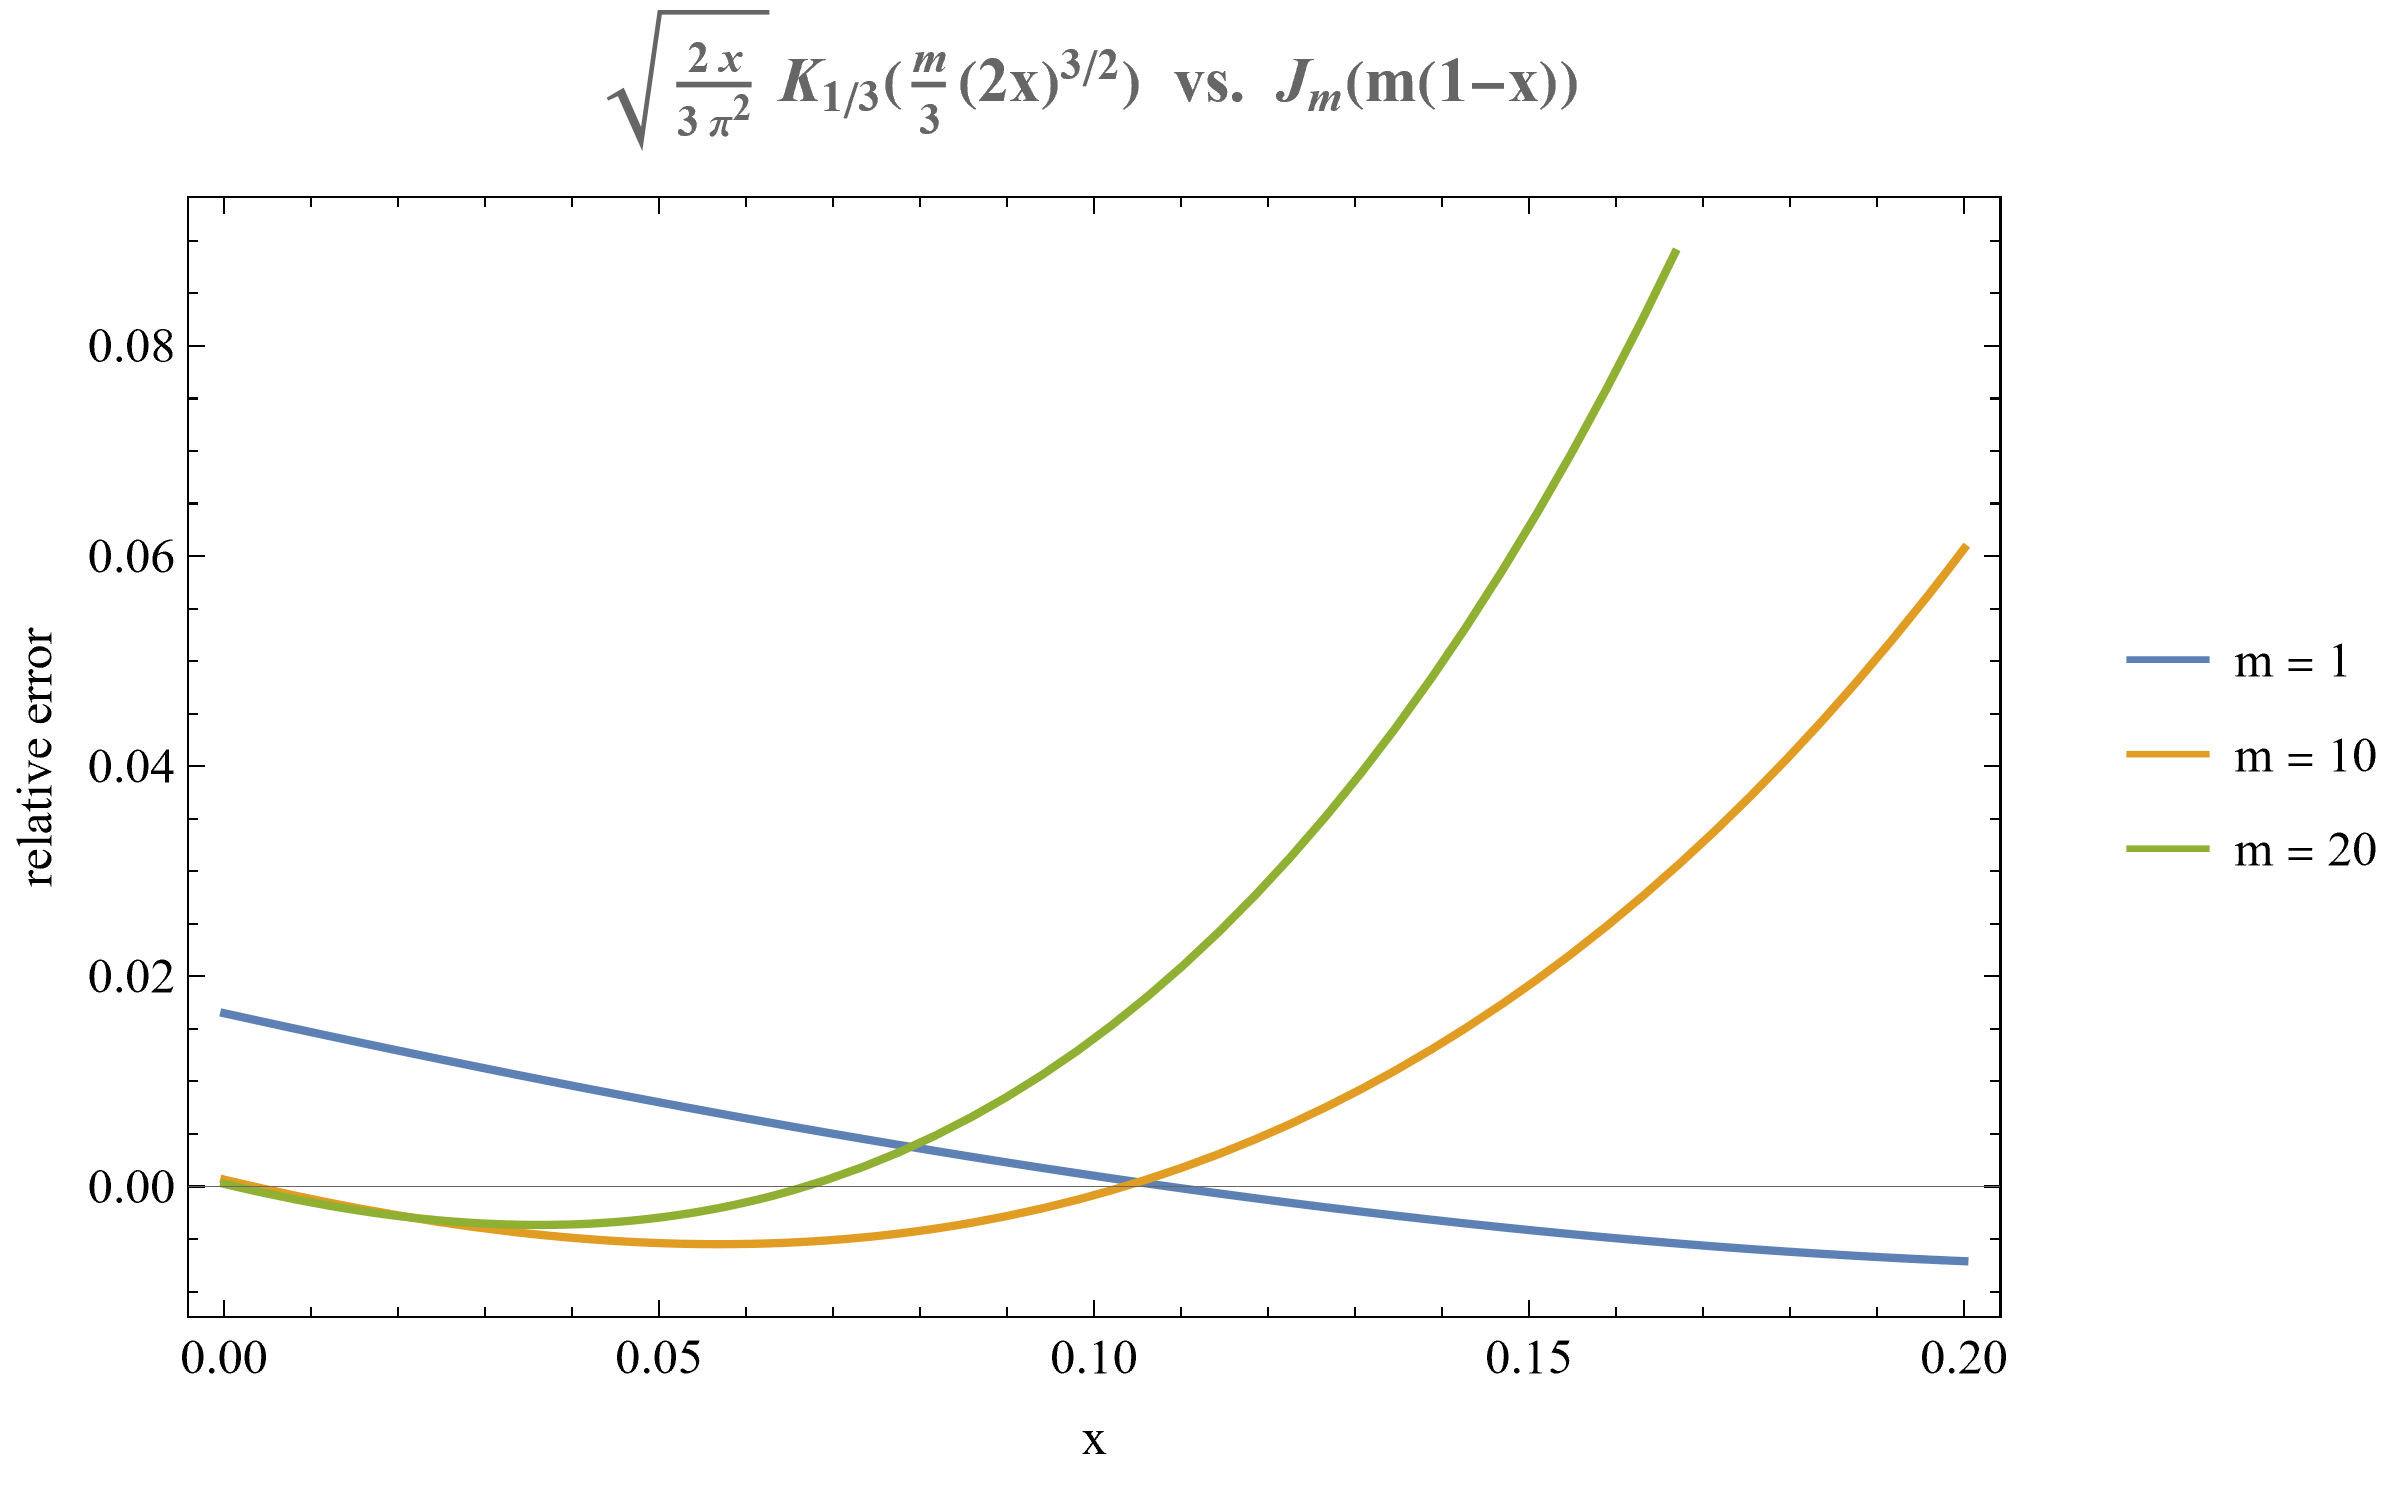
\includegraphics[width=0.49\textwidth]{special_functions_fig/airy_type_function_asymptotic_comparison.png}
	\caption{Airy型函数渐近式比较}
	\label{Airy型函数渐近式比较}
\end{figure}

与立方电阻网有关的公式\(|m| \leq l,\,m \in \mathbb{Z}\)
\begin{equation*}
	&\dfrac{1}{l} \sum_{k=0}^{l-1} \dfrac{\sin\left( \dfrac{2\pi k m}{l} \right)}{A - \cos\left( \dfrac{2\pi k}{l} \right)} = 0,\quad \dfrac{1}{l} \sum_{k=0}^{l-1} \dfrac{1 - \cos\left( \dfrac{2\pi k m}{l} \right)}{1 - \cos\left( \dfrac{2\pi k}{l} \right)} = |m|.\\
	&\dfrac{1}{l} \sum_{k=0}^{l-1} \dfrac{\cos\left( \dfrac{2\pi k m}{l} \right)}{A - \cos\left( \dfrac{2\pi k}{l} \right)} = \dfrac{1}{\sqrt{A^2 - 1}} \cdot \dfrac{(A - \sqrt{A^2 - 1})^{|m|} - (A - \sqrt{A^2 - 1})^{l - |m|}}{1 - (A - \sqrt{A^2 - 1})^l}.
\end{equation*}

与柱对称混合边界条件有关的方程解
\begin{equation*}
&\int_0^\infty y f(y) J_\nu(yx) \,\mathrm{d}y = x^\nu, \quad x < 1. \qquad
\int_0^\infty f(y) J_\nu(yx) \,\mathrm{d}y = 0, \quad x \ge 1.\\
&\implies\quad f(y) = \frac{\Gamma(\nu+1)}{\sqrt{\pi}\,\Gamma\left(\nu+\dfrac{3}{2}\right)} j_{\nu+1}(y) = \frac{\Gamma(\nu+1)}{\sqrt{2y}\,\Gamma\left(\nu+\dfrac{3}{2}\right)} J_{\nu+\frac{3}{2}}(y).\\
\\
&\int_0^\infty g(y) J_\nu(yx) \,\mathrm{d}y = x^\nu, \quad x < 1. \qquad
\int_0^\infty y g(y) J_\nu(yx) \,\mathrm{d}y = 0, \quad x \ge 1.\\
&\implies\quad g(y) = \frac{2\Gamma(\nu+1)}{\sqrt{\pi}\,\Gamma\left(\nu+\dfrac{1}{2}\right)} j_{\nu}(y) = \frac{\Gamma(\nu+1)}{\Gamma\left(\nu+\dfrac{1}{2}\right)}\sqrt{\frac{2}{y}}\,J_{\nu+\frac{1}{2}}(y).
\end{equation*}

\end{document}